% Options for packages loaded elsewhere
\PassOptionsToPackage{unicode}{hyperref}
\PassOptionsToPackage{hyphens}{url}
%
\documentclass[
  ignorenonframetext,
]{beamer}
\usepackage{pgfpages}
\setbeamertemplate{caption}[numbered]
\setbeamertemplate{caption label separator}{: }
\setbeamercolor{caption name}{fg=normal text.fg}
\beamertemplatenavigationsymbolsempty
% Prevent slide breaks in the middle of a paragraph
\widowpenalties 1 10000
\raggedbottom
\setbeamertemplate{part page}{
  \centering
  \begin{beamercolorbox}[sep=16pt,center]{part title}
    \usebeamerfont{part title}\insertpart\par
  \end{beamercolorbox}
}
\setbeamertemplate{section page}{
  \centering
  \begin{beamercolorbox}[sep=12pt,center]{part title}
    \usebeamerfont{section title}\insertsection\par
  \end{beamercolorbox}
}
\setbeamertemplate{subsection page}{
  \centering
  \begin{beamercolorbox}[sep=8pt,center]{part title}
    \usebeamerfont{subsection title}\insertsubsection\par
  \end{beamercolorbox}
}
\AtBeginPart{
  \frame{\partpage}
}
\AtBeginSection{
  \ifbibliography
  \else
    \frame{\sectionpage}
  \fi
}
\AtBeginSubsection{
  \frame{\subsectionpage}
}
\usepackage{amsmath,amssymb}
\usepackage{iftex}
\ifPDFTeX
  \usepackage[T1]{fontenc}
  \usepackage[utf8]{inputenc}
  \usepackage{textcomp} % provide euro and other symbols
\else % if luatex or xetex
  \usepackage{unicode-math} % this also loads fontspec
  \defaultfontfeatures{Scale=MatchLowercase}
  \defaultfontfeatures[\rmfamily]{Ligatures=TeX,Scale=1}
\fi
\usepackage{lmodern}
\usetheme[]{Berlin}
\usecolortheme{beaver}
\usefonttheme{structurebold}
\ifPDFTeX\else
  % xetex/luatex font selection
\fi
% Use upquote if available, for straight quotes in verbatim environments
\IfFileExists{upquote.sty}{\usepackage{upquote}}{}
\IfFileExists{microtype.sty}{% use microtype if available
  \usepackage[]{microtype}
  \UseMicrotypeSet[protrusion]{basicmath} % disable protrusion for tt fonts
}{}
\makeatletter
\@ifundefined{KOMAClassName}{% if non-KOMA class
  \IfFileExists{parskip.sty}{%
    \usepackage{parskip}
  }{% else
    \setlength{\parindent}{0pt}
    \setlength{\parskip}{6pt plus 2pt minus 1pt}}
}{% if KOMA class
  \KOMAoptions{parskip=half}}
\makeatother
\usepackage{xcolor}
\newif\ifbibliography
\usepackage{longtable,booktabs,array}
\usepackage{calc} % for calculating minipage widths
\usepackage{caption}
% Make caption package work with longtable
\makeatletter
\def\fnum@table{\tablename~\thetable}
\makeatother
\usepackage{graphicx}
\makeatletter
\def\maxwidth{\ifdim\Gin@nat@width>\linewidth\linewidth\else\Gin@nat@width\fi}
\def\maxheight{\ifdim\Gin@nat@height>\textheight\textheight\else\Gin@nat@height\fi}
\makeatother
% Scale images if necessary, so that they will not overflow the page
% margins by default, and it is still possible to overwrite the defaults
% using explicit options in \includegraphics[width, height, ...]{}
\setkeys{Gin}{width=\maxwidth,height=\maxheight,keepaspectratio}
% Set default figure placement to htbp
\makeatletter
\def\fps@figure{htbp}
\makeatother
\setlength{\emergencystretch}{3em} % prevent overfull lines
\providecommand{\tightlist}{%
  \setlength{\itemsep}{0pt}\setlength{\parskip}{0pt}}
\setcounter{secnumdepth}{-\maxdimen} % remove section numbering
% definitions for citeproc citations
\NewDocumentCommand\citeproctext{}{}
\NewDocumentCommand\citeproc{mm}{%
  \begingroup\def\citeproctext{#2}\cite{#1}\endgroup}
\makeatletter
 % allow citations to break across lines
 \let\@cite@ofmt\@firstofone
 % avoid brackets around text for \cite:
 \def\@biblabel#1{}
 \def\@cite#1#2{{#1\if@tempswa , #2\fi}}
\makeatother
\newlength{\cslhangindent}
\setlength{\cslhangindent}{1.5em}
\newlength{\csllabelwidth}
\setlength{\csllabelwidth}{3em}
\newenvironment{CSLReferences}[2] % #1 hanging-indent, #2 entry-spacing
 {\begin{list}{}{%
  \setlength{\itemindent}{0pt}
  \setlength{\leftmargin}{0pt}
  \setlength{\parsep}{0pt}
  % turn on hanging indent if param 1 is 1
  \ifodd #1
   \setlength{\leftmargin}{\cslhangindent}
   \setlength{\itemindent}{-1\cslhangindent}
  \fi
  % set entry spacing
  \setlength{\itemsep}{#2\baselineskip}}}
 {\end{list}}
\usepackage{calc}
\newcommand{\CSLBlock}[1]{\hfill\break\parbox[t]{\linewidth}{\strut\ignorespaces#1\strut}}
\newcommand{\CSLLeftMargin}[1]{\parbox[t]{\csllabelwidth}{\strut#1\strut}}
\newcommand{\CSLRightInline}[1]{\parbox[t]{\linewidth - \csllabelwidth}{\strut#1\strut}}
\newcommand{\CSLIndent}[1]{\hspace{\cslhangindent}#1}
\setbeamertemplate{navigation symbols}{}
\setbeamertemplate{footline}[page number]
\ifLuaTeX
  \usepackage{selnolig}  % disable illegal ligatures
\fi
\usepackage{bookmark}
\IfFileExists{xurl.sty}{\usepackage{xurl}}{} % add URL line breaks if available
\urlstyle{same}
\hypersetup{
  pdftitle={Inferential Capabilities of Multillevel Weibull Regression for the Psychological Sciences},
  pdfauthor={Adon Rosen},
  hidelinks,
  pdfcreator={LaTeX via pandoc}}

\title{Inferential Capabilities of Multillevel Weibull Regression for
the Psychological Sciences}
\author{Adon Rosen}
\date{June 4th 2024}
\institute{University of Oklahoma}

\begin{document}
\frame{\titlepage}

\section{Background}\label{background}

\begin{frame}{Outline}
\phantomsection\label{outline}
\begin{enumerate}
\tightlist
\item
  Background:

  \begin{enumerate}
  \tightlist
  \item
    Time-series analysis in the behavioral sciences
  \item
    The Markov model
  \item
    Survival Analysis
  \item
    The similarities of Markov models and Survival Analysis
  \end{enumerate}
\item
  Simulation study
\item
  Empirical study
\item
  Conclusions
\end{enumerate}
\end{frame}

\begin{frame}{Psychological Time-series Data}
\phantomsection\label{psychological-time-series-data}
\begin{enumerate}
\item
  Acquiring time-series data for the psychological sciences is easier
  now than ever before.
\item
  Techniques such as Ecological Momentary Assessment have made the
  acquisition of these data easier now than ever before (Shiffman,
  Stone, and Hufford 2008)
\end{enumerate}
\end{frame}

\begin{frame}{Analysis of Time-series Example}
\phantomsection\label{analysis-of-time-series-example}
\begin{longtable}[]{@{}lll@{}}
\toprule\noalign{}
Time & Data & Potential Methods \\
\midrule\noalign{}
\endhead
Discrete (A) & Discrete & \textbf{Markov model} \\
Discrete (B) & Continuous & Auto regressive model \\
Continuous (C) & Discrete & \textbf{Continuous-time Markov model} \\
Continuous (D) & Continuous & Differential Equations \\
\bottomrule\noalign{}
\end{longtable}

\includegraphics{dissertationPres_files/figure-beamer/stateExamp-1.pdf}
\end{frame}

\begin{frame}{What is a Markov Model}
\phantomsection\label{what-is-a-markov-model}
Markov models are composed of two components:

\begin{enumerate}
\item
  A set of states: \(S={S_1, S_2, ..., S_r}\)
\item
  A set of transitions between the states, \(p_{ij}\), which forms the
  markov transition matrix:

  \begin{enumerate}
  \tightlist
  \item
    \(\begin{array}{ccc} &\begin{array}{cccc} S_{1} & S_{2}\end{array}\\P=\begin{array}{cccc}S_{1} \\S_{2} \\\end{array}&\left(\begin{array}{cccc}p_{11} & p_{12}  \\p_{21} & p_{22}  \\\end{array}\right)\end{array}\)
  \end{enumerate}
\end{enumerate}

Assumptions of the Markov model include:

\begin{enumerate}
\item
  The system exists in one and only one of the states at all times
\item
  The system makes a transition from one state to another

  \begin{enumerate}
  \item
    Transitions can be made in continuous or discrete-time
  \item
    Discrete-time transitions are made when transitions are performed in
    unit values
  \item
    Continuous-time transitions can occur at any real-valued time
    interval
  \end{enumerate}
\end{enumerate}
\end{frame}

\begin{frame}{Additional Markov model assumptions}
\phantomsection\label{additional-markov-model-assumptions}
\begin{enumerate}
\tightlist
\item
  The first assumption states that the probability of future
  transitions\\
  is only influenced by the current state of the system

  \begin{enumerate}
  \tightlist
  \item
    \(P(X_{t+1}= j | X_{t} = i, X_{t-1} = ..., X1) = P(X_{t+1} = j | X_t = i)\)
  \end{enumerate}
\item
  The second assumption, the \emph{memoryless} property for a
  continuous-time Markov model is details how transition intensities are
  static across time.

  \begin{enumerate}
  \tightlist
  \item
    \(q_{ij}(t,z(t)) = lim_{\Delta t\rightarrow0} \frac{P(S(t+ \Delta t) = s|S(t) = r)}{\Delta t}\)
  \end{enumerate}
\end{enumerate}
\end{frame}

\begin{frame}{How have Markov Models been used for Psychological
Research}
\phantomsection\label{how-have-markov-models-been-used-for-psychological-research}
The Markov model has been a mainstay analytic tool in the psychological
sciences for the last 80 years.

The first application was used by Robert Miller in 1952 who used to
Markov model to estimate rats learning progression when navigating a
``T'' maze (Miller 1952)

The Markov model has grown in popularity and has been applied across a
wide range of fields includes:

drug use: Lee et al.~(2018)

resilience research: von Eye \& Brandstädter (1998); von Eye \&
Schuster, 2000)

interpersonal dynamics: Li et al., 2020

personality research: de Haan-Rietdijk et al., (2017)

measurement invariance of EMA Vogelsmeier et al., (2022)

All of these examples apply a discrete-time approach towards the
application of the Markov model.
\end{frame}

\begin{frame}{Background on Survival Analysis}
\phantomsection\label{background-on-survival-analysis}
\begin{columns}[T]
\begin{column}{0.6\textwidth}
Survival analysis seeks to predict the probability of an event occurring
at a specific point in time.

The most commonly applied technique to analyze survival data is the
Kaplan-Meier approach (Kaplan and Meier 1958)

The Kaplan-Meier approach is a nonparametric that can be used to
estimate hazards

It has different names depending on the field that is applying it:
survival analysis (epidemiology); reliability analysis or
\textbf{time-to-event} (engineering); event history analysis (sociology)
\end{column}

\begin{column}{0.4\textwidth}
\includegraphics{dissertationPres_files/figure-beamer/simSurvDat-1.pdf}
\end{column}
\end{columns}
\end{frame}

\begin{frame}{Background on time-to-event cont.}
\phantomsection\label{background-on-time-to-event-cont.}
\begin{columns}[T]
\begin{column}{0.4\textwidth}
\includegraphics{dissertationPres_files/figure-beamer/survExample-1.pdf}
\end{column}

\begin{column}{0.6\textwidth}
\begin{itemize}
\item
  Density:\\
  \(h(t) = lim_{\Delta t \rightarrow0}\frac{P(t\leq T < t + \Delta t | T \geq t)}{\Delta t}\)
\item
  Cumulative:\\
  \(F(t) = \int_{0}^{t} f(u) du = P(T < t)\)
\item
  Survival:\\
  \(S(t) = 1 - F(t)\)
\item
  Density*:\\
  \(h(t) = \frac{f(t)}{S(t)}\)
\end{itemize}
\end{column}
\end{columns}
\end{frame}

\begin{frame}{Background on time-to-event cont.}
\phantomsection\label{background-on-time-to-event-cont.-1}
Together these functions can be used to identify whether or when an
event is likely to occur given the current state of an individual
(Keiley and Martin 2005)

Two additional benefits of survival analysis makes them powerful
analytic tools:

\begin{enumerate}
\item
  Inferential capabilities
\item
  Multilevel modeling
\end{enumerate}
\end{frame}

\begin{frame}{Inference in time-to-event Analysis}
\phantomsection\label{inference-in-time-to-event-analysis}
\begin{enumerate}
\item
  Predictive variables can be incorporated to examine variables that
  predict the hazards

  \begin{enumerate}
  \item
    Inference in survival analysis is most popularly assessed via the
    Cox Proportional Hazards (Cox PH) model (Cox 1972)
  \item
    The model takes the following form:

    \begin{enumerate}
    \tightlist
    \item
      \(h(t|X_i)=h_0(t)e^{\beta X_i}\)
    \end{enumerate}
  \end{enumerate}
\end{enumerate}

\includegraphics{dissertationPres_files/figure-beamer/survPlotME-1.pdf}
\end{frame}

\begin{frame}{Accommodating clusters in time-to-event analysis (frailty
modeling)}
\phantomsection\label{accommodating-clusters-in-time-to-event-analysis-frailty-modeling}
\begin{enumerate}
\tightlist
\item
  Frailty models are extensions survival models
\item
  The effects of \textbf{unobserved heterogeneity} on life times are
  collectively referred to as \emph{frailty} in demographic research.
  (Balan and Putter 2020)
\item
  Frailty models can also be used to model dependence of survival times
  in clustered data or recurrent events
\item
  An additional term is included when estimating the hazards of an
  individual that belongs to a specific group

  \begin{enumerate}
  \tightlist
  \item
    Frailty hazards: \(h(t|Z)=Zh(t)\)
  \end{enumerate}
\end{enumerate}
\end{frame}

\begin{frame}{Accommodating clusters in time-to-event analysis (frailty
modeling) cont.}
\phantomsection\label{accommodating-clusters-in-time-to-event-analysis-frailty-modeling-cont.}
\includegraphics[width=\textwidth,height=2.29167in]{images/clipboard-1947213930.png}

(Lougheed et al. 2019)
\end{frame}

\begin{frame}{Parametric time-to-event analysis}
\phantomsection\label{parametric-time-to-event-analysis}
\begin{columns}[T]
\begin{column}{0.7\textwidth}
While the Kaplan-Meier is arguably the most popular technique used to
analyze time-to-event data, alternative fully parametric techniques also
exist which can be used to estimate hazards

Examples of fully parametric time-to-event technique include
\textbf{Weibull regression}, and the more commonly applied
\textbf{Exponential regression}
\end{column}

\begin{column}{0.3\textwidth}
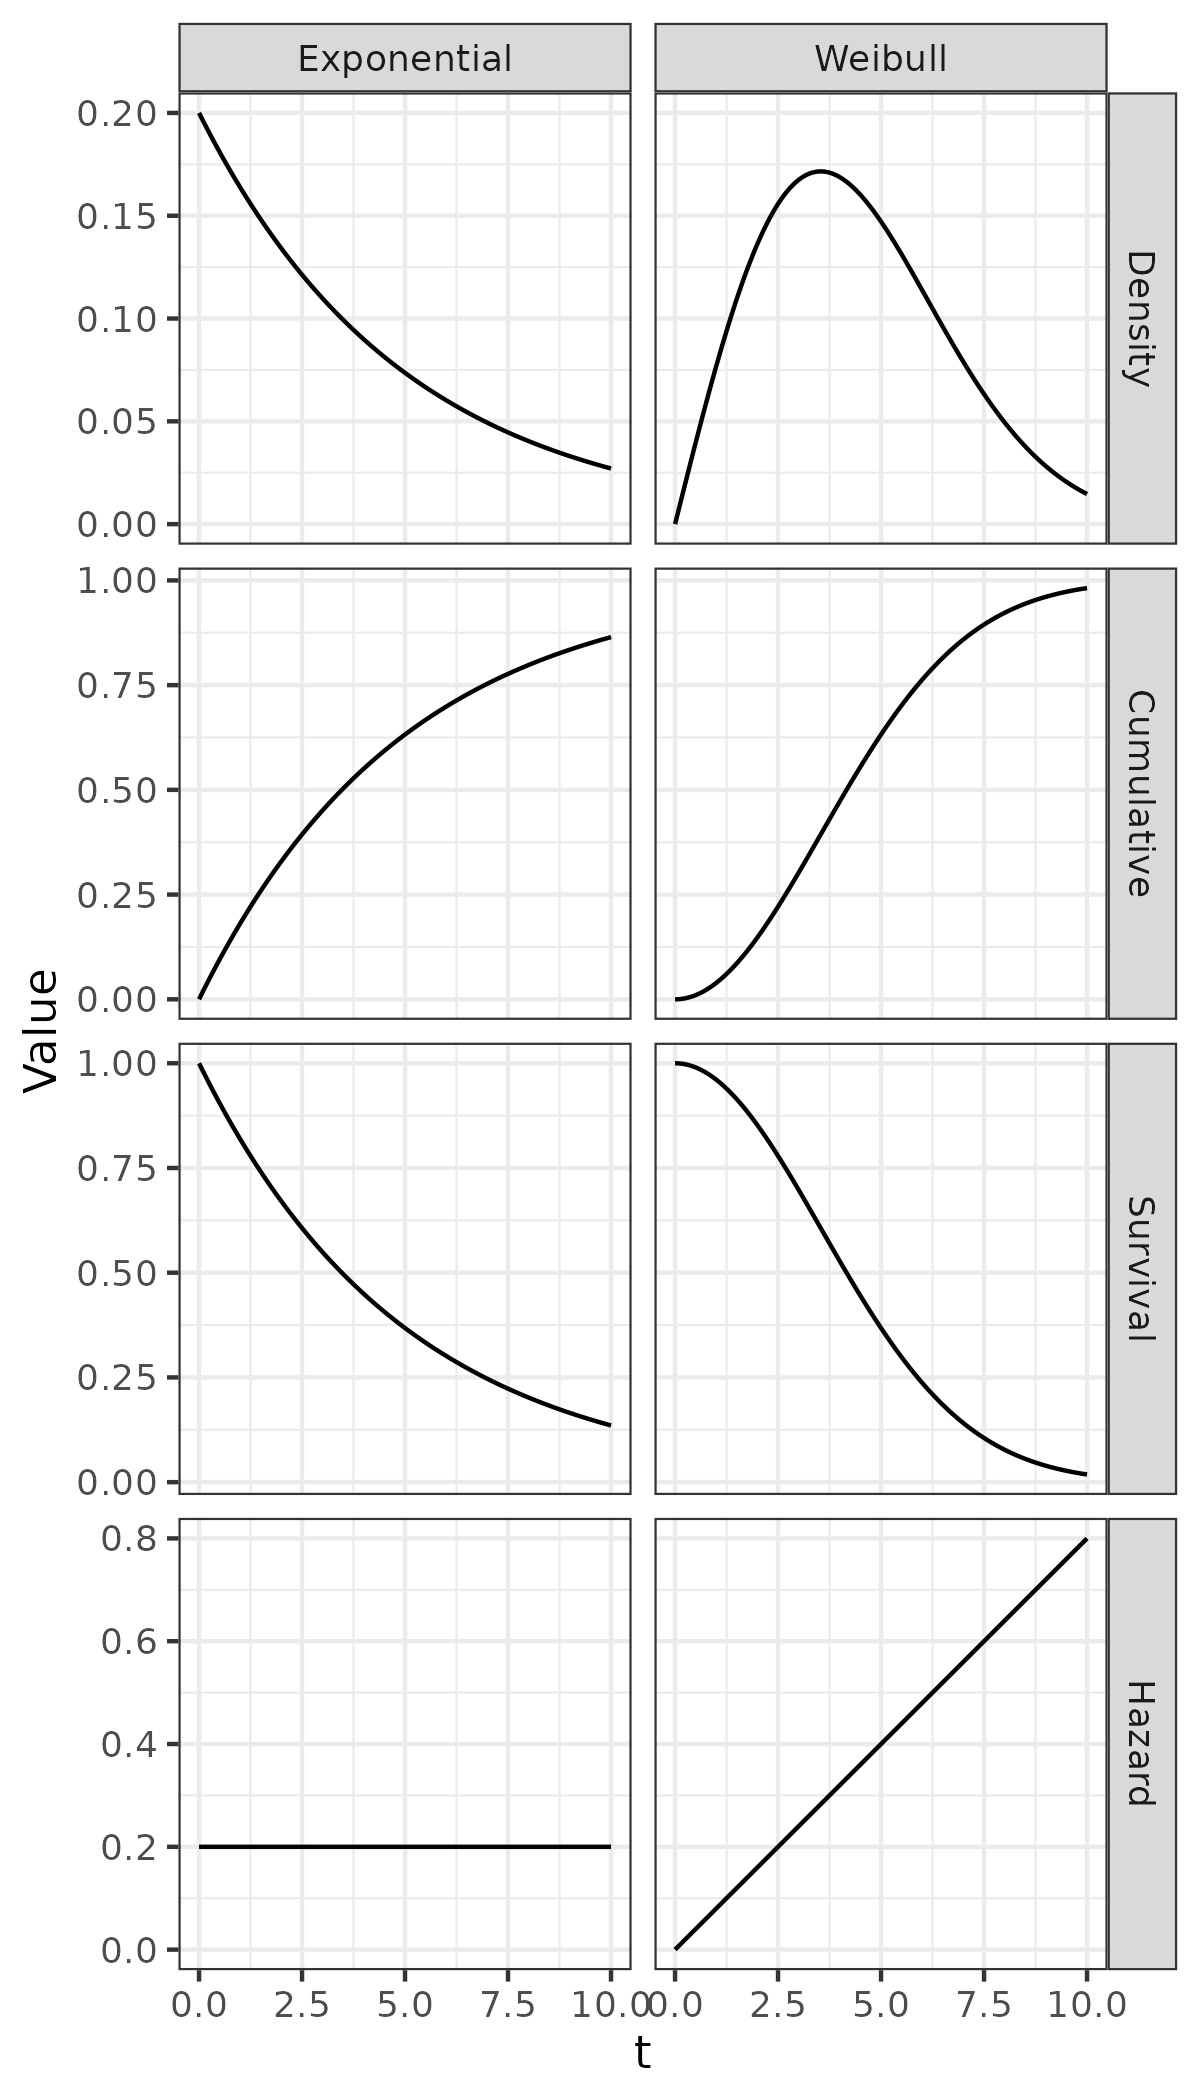
\includegraphics{figures/weiExpFig.png}
\end{column}
\end{columns}
\end{frame}

\begin{frame}{Parametric time-to-event analysis cont.}
\phantomsection\label{parametric-time-to-event-analysis-cont.}
\begin{columns}[T]
\begin{column}{0.7\textwidth}
\begin{table}
    \centering
    \begin{tabular}{ccc}
        Function & Exponential & Weibull \\
        f(t) & \(\lambda e^{-\lambda t}\) &
\(\lambda\gamma t^{\gamma-1}e^{-\lambda t^{\gamma}}\) \\
        S(t) & \(e^{-\lambda t}\) & \(e^{-\lambda t^\gamma}\) \\
        h(t) & \(\lambda\) & \(\lambda \gamma ^{\gamma - 1}\) \\
    \end{tabular}
\end{table}
\end{column}

\begin{column}{0.3\textwidth}
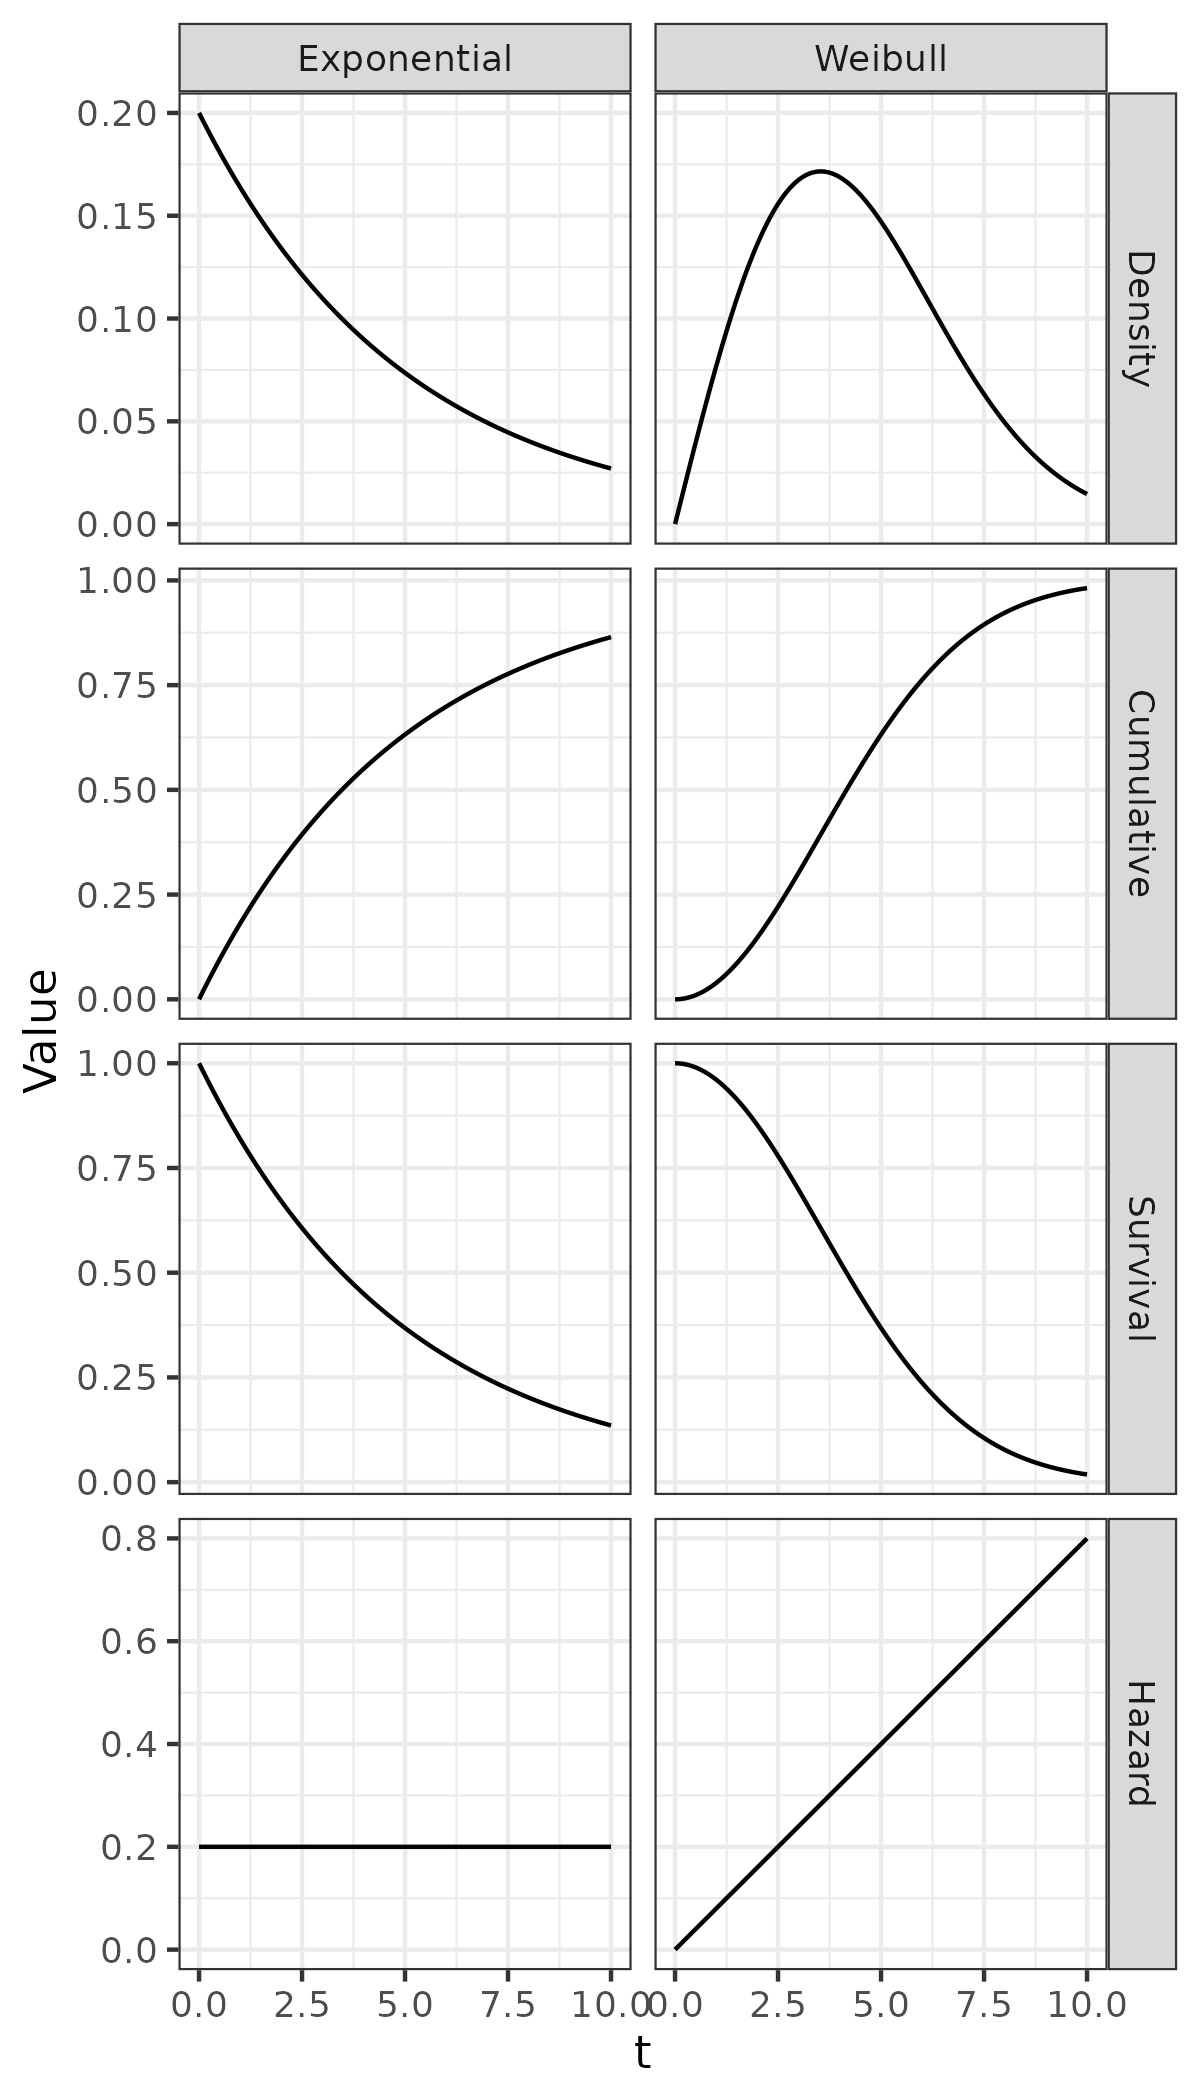
\includegraphics[width=\textwidth,height=2.29167in]{figures/weiExpFig.png}
\end{column}
\end{columns}
\end{frame}

\begin{frame}{Weibull Regression.}
\phantomsection\label{weibull-regression.}
\begin{columns}[T]
\begin{column}{0.6\textwidth}
\begin{enumerate}
\tightlist
\item
  Weibull regression works in a linear capacity using the following
  transformation:

  \begin{enumerate}
  \tightlist
  \item
    \(F(t) = 1 - exp[(-(t/\lambda)^\gamma)]\)
  \item
    \(ln(t) = ln(\gamma) + (\frac{1}{\lambda})ln(ln(\frac{1}{1-F}))\)
  \item
    This builds a linear regression \(Y=A+BX\) framework:

    \begin{enumerate}
    \tightlist
    \item
      Y = \(ln(t)\)
    \item
      X = \(ln(ln(1/(1-F)))\)
    \item
      A = \(\ln{\gamma}\)
    \item
      B = \(\frac{1}{\lambda}\)
    \end{enumerate}
  \end{enumerate}
\end{enumerate}
\end{column}

\begin{column}{0.4\textwidth}
\includegraphics{images/clipboard-3457825580.png}
\end{column}
\end{columns}
\end{frame}

\begin{frame}{Background on semi-Markov models}
\phantomsection\label{background-on-semi-markov-models}
\begin{columns}[T]
\begin{column}{0.5\textwidth}
\begin{enumerate}
\tightlist
\item
  Semi-Markov models loosen the \emph{memoryless} assumption of the
  Markov model and can incorporate a ``local clock'' which influences
  the transition intensities across states.
\item
  A local clock describes the time a unit has spent in the current state
\end{enumerate}
\end{column}

\begin{column}{0.5\textwidth}
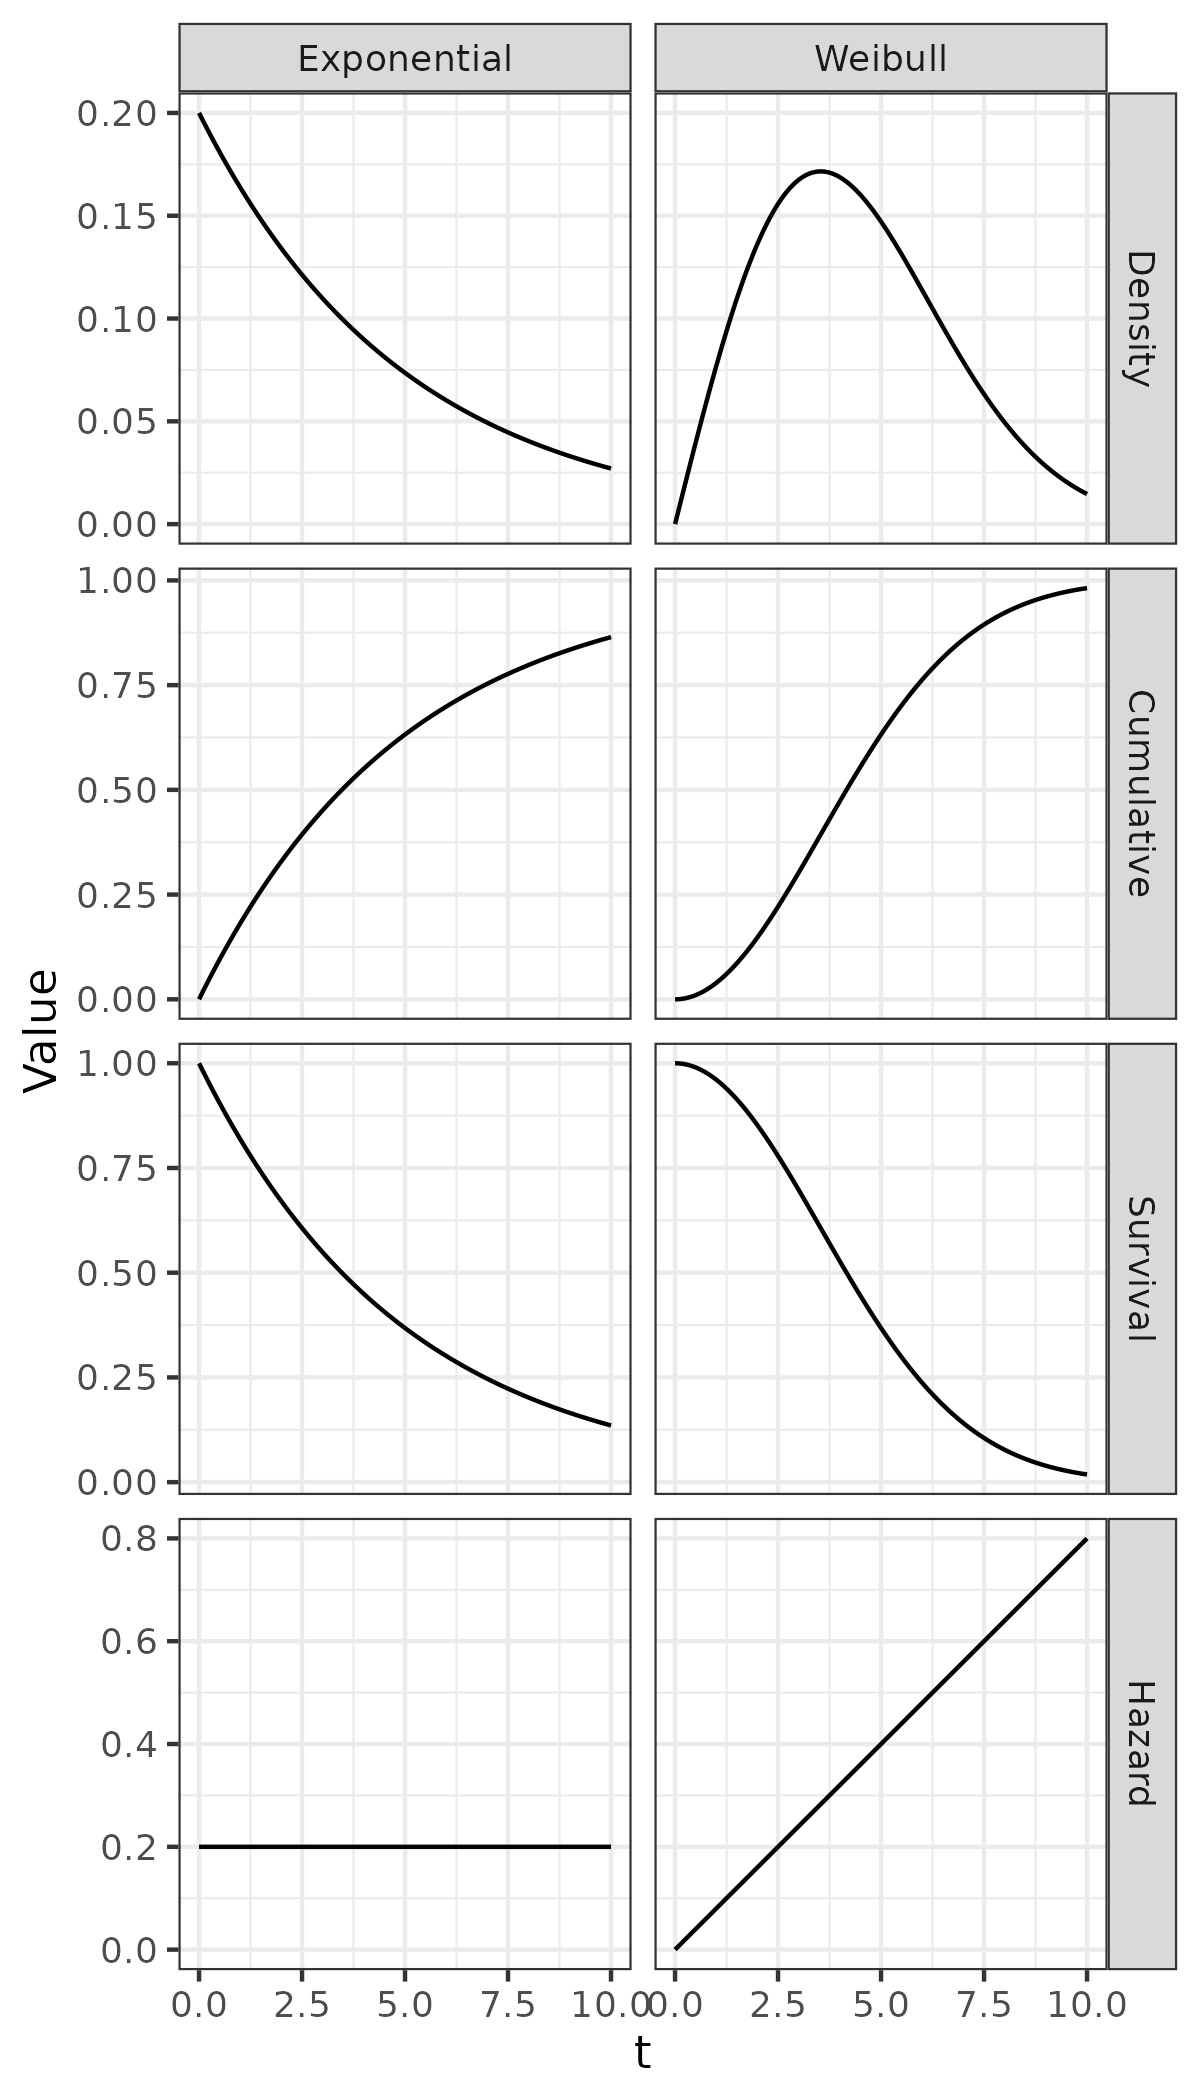
\includegraphics[width=\textwidth,height=2.29167in]{figures/weiExpFig.png}
\end{column}
\end{columns}
\end{frame}

\begin{frame}{Estimation of a semi-Markov model}
\phantomsection\label{estimation-of-a-semi-markov-model}
Estimating a semi-Markov model requires identifying the transition
intensities from one state into another:

Density:
\(h_{ij}(t) = lim_{\Delta t \rightarrow0}\frac{P(t\leq T < t + \Delta t | T \geq t)}{\Delta t}\)

Cumulative: \(F_{ij}(t) = \int_{0}^{t} f(u) du = P(T < t)\)

Survival: \(S_{ij}(t) = 1 - F(t)\)

\textbf{The semi-Markov model allows for functions outside of the
exponential distribution to be used to model transitions across states}

The fully parametric Weibull regression can be used to estimate
semi-Markov models
\end{frame}

\begin{frame}{The similarity of Markov models and survival analysis}
\phantomsection\label{the-similarity-of-markov-models-and-survival-analysis}
\begin{enumerate}
\item
  Translating between a time-to-event analysis and a semi-Markov can be
  done with the following equality:

  \(h(t)_{ij}=\frac{p_{ij}S_{ij}(t)}{S_{i}(t)}f_{ij}(t)=p_{ij}\frac{f_{ij}(t)}{S_i(t)}\)
\item
  A multi-state Weibull model can be translated into a semi-Markov model
  with:
  \(h_{ij}(t)=p_{ij}\frac{\gamma_{ij}}{\lambda_{ij}}(\frac{t}{\lambda_{ij}})^{\gamma_{ij}-1}=\frac{\gamma_{ij}}{p_{ij}^{-1/\gamma_{ij}}\lambda_{ij}}(\frac{t}{p_{ij}^{-1/\gamma_{ij}}\lambda_{ij}})^{\gamma_{ij}-1}\)
\end{enumerate}
\end{frame}

\begin{frame}{Review}
\phantomsection\label{review}
\begin{enumerate}
\tightlist
\item
  Markov models are a commonly applied technique used to study
  discrete-state time-series data
\item
  The Markov assumption however may restrict the utility of the model
  for behavioral data, it is too restrictive of an assumption to assume
  that transitions across states are static for the behavioral sciences
\item
  A multi-state Weibull regression model can be used to identify hazards
  that are not static overtime
\item
  Additionally the Weibull regression model can incorporate frailty
  terms, can be used for statistical inference, and can be used to
  translate findings into semi-Markov models
\end{enumerate}
\end{frame}

\begin{frame}{Problem statement}
\phantomsection\label{problem-statement}
\begin{enumerate}
\tightlist
\item
  Given the popularity of the Markov model, three questions now arise:

  \begin{enumerate}
  \tightlist
  \item
    How well does the Markov model perform when the model's assumptions
    are not met?
  \item
    How well does the Markov model perform when population heterogeneity
    does exist?
  \item
    Does the semi-Markov model outperform the Markov model in data that
    are reflective of psychological studies?
  \end{enumerate}
\end{enumerate}
\end{frame}

\section{Simulation}\label{simulation}

\begin{frame}{Motivation}
\phantomsection\label{motivation}
The simulation study was motivated by two questions:

\begin{enumerate}
\item
  How well does the Markov model perform when data do not adhere to the
  assumptions of the Markov model?
\item
  How well do the fixed effect models perform when there is population
  heterogeneity \& can a random effect mitigate potential heterogeneity
  concerns?
\end{enumerate}

In order to address these questions a simulation study was performed to
examine how well the Markov and the semi-Markov model perform under
various simulation characteristics.
\end{frame}

\begin{frame}{Methods}
\phantomsection\label{methods}
1,000 data sets were generated by sampling sojourn times from Weibull
distributions under varying 8 sampling characteristics, factors were
fully crossed yielding a total of 128,000 unique data sets. The factors
included

\begin{enumerate}
\item
  Sample Size (20 \textbar{} 100)
\item
  Observation Length (20 \textbar{} 40)
\item
  Transition Matrix (Stable \textbar{} Random)
\item
  Weibull Scale Range (.5-5 \textbar{} 5-10)
\item
  Weibull Shape Parameter (1 \textbar{} 3)
\item
  \textbf{Criterion Variable Magnitude (Null \textbar{} Large)}
\item
  \textbf{Random Effect Variance (0 \textbar{} 1)}
\item
  \textbf{Modeling Strategy}
\end{enumerate}
\end{frame}

\begin{frame}{Sample Size}
\phantomsection\label{sample-size}
Sample size determines the number of unique individuals that provide
data.

Larger sample sizes are almost always more desirable and will increase
inferential power.

\begin{block}{}
\phantomsection\label{section}
\includegraphics{images/sampleSize-01.png}
\end{block}
\end{frame}

\begin{frame}{Observation Length}
\phantomsection\label{observation-length}
Longer observation periods provide more information both about an
individual's heterogeneity and the sampling characteristics of the true
Weibull distribution.

\begin{block}{}
\phantomsection\label{section-1}
\includegraphics{images/sampleLength.png}
\end{block}
\end{frame}

\begin{frame}{Transition matrix}
\phantomsection\label{transition-matrix}
A more stable transition matrix provides less information about
inter-state transitions, making estimation of true Weibull
characteristics more difficult

\begin{block}{}
\phantomsection\label{section-2}
\includegraphics{images/stateEmissonRand.png}
\end{block}
\end{frame}

\begin{frame}{Weibull characteristics}
\phantomsection\label{weibull-characteristics}
A two-parameter Weibull distribution was used to sample sojourn times.
The two-parameter Weibull function is composed of a shape and a scale
parameter.

\includegraphics{dissertationPres_files/figure-beamer/distFuns-1.pdf}
\end{frame}

\begin{frame}{Criterion variable magnitude}
\phantomsection\label{criterion-variable-magnitude}
\begin{enumerate}
\tightlist
\item
  A population fixed effect variable of interest (criterion variable)
  will take two either a null effect (0) or a large magnitude effect
  (0.8)
\item
  This variable will take the form of a time- invariant predictor
  generated from a normal distribution N(0,1)
\end{enumerate}
\end{frame}

\begin{frame}{Random effect variance}
\phantomsection\label{random-effect-variance}
\begin{enumerate}
\tightlist
\item
  Two levels were selected: none \& large random variance
\item
  The major motivation is to simulate ``stayer'' and ``movers''
\end{enumerate}

\includegraphics{dissertationPres_files/figure-beamer/varExamp-1.pdf}
\end{frame}

\begin{frame}{Modeling Strategy}
\phantomsection\label{modeling-strategy}
\begin{enumerate}
\tightlist
\item
  Four models were estimated for every simulated dataset
\item
  The four models include:

  \begin{enumerate}
  \tightlist
  \item
    Continuous-time Markov model (exponential):
  \item
    Multilevel continuous-time Markov model (exponential)
  \item
    Continuous-time semi-Markov model (Weibull)
  \item
    \textbf{Multilevel continuous-time semi-Markov model (Weibull)}
  \end{enumerate}
\item
  Every model included fixed effects for the type of transitions and the
  criterion variable; the multilevel model included a random intercept
  term
\item
  All models were estimated using a Bayesian framework; naive and
  diffuse priors were used to estimate every model

  \begin{enumerate}
  \tightlist
  \item
    5000 chains; 2000 warmup; thinning of 5; four chains were estimated
  \item
    Sampling was performed using the NUTS algorithm implemented in the
    STAN language (Team 2023)
  \end{enumerate}
\end{enumerate}
\end{frame}

\begin{frame}{Simulation Outcomes}
\phantomsection\label{simulation-outcomes}
\begin{enumerate}
\tightlist
\item
  The simulation examined four outcomes:

  \begin{enumerate}
  \tightlist
  \item
    Estimation error of the criterion variable
  \item
    Estimation error of the shape parameter*
  \item
    Examine criterion variable error specific to shape error*
  \item
    Criterion variable coverage
  \end{enumerate}
\item
  An ANOVA model was used for outcomes 1 \& 2;
\item
  An ANCOVA was used for outcome 3
\item
  A logistic model was used for outcome 4
\item
  \textbf{Outcomes 2 \& 3 were limited to semi-Markov models}
\end{enumerate}
\end{frame}

\begin{frame}{Results question 1}
\phantomsection\label{results-question-1}
\begin{enumerate}
\tightlist
\item
  Q1 examines the difference between the estimated and true criterion
  variable
\end{enumerate}

\begin{table}
    \centering
    \begin{tabular}{cc}
        Parameter & \(\eta^2\) \\
        Magnitude of Random Variance & .29 \\
        Sample Size & .15\\
        Model Strategy & .05 \\
        Sample Size: Magnitude of Random Variance & .10 \\
        Model Strategy: Magnitude of Random Variance & .03 \\
    \end{tabular}
\end{table}
\end{frame}

\begin{frame}{Results question 1}
\phantomsection\label{results-question-1-1}
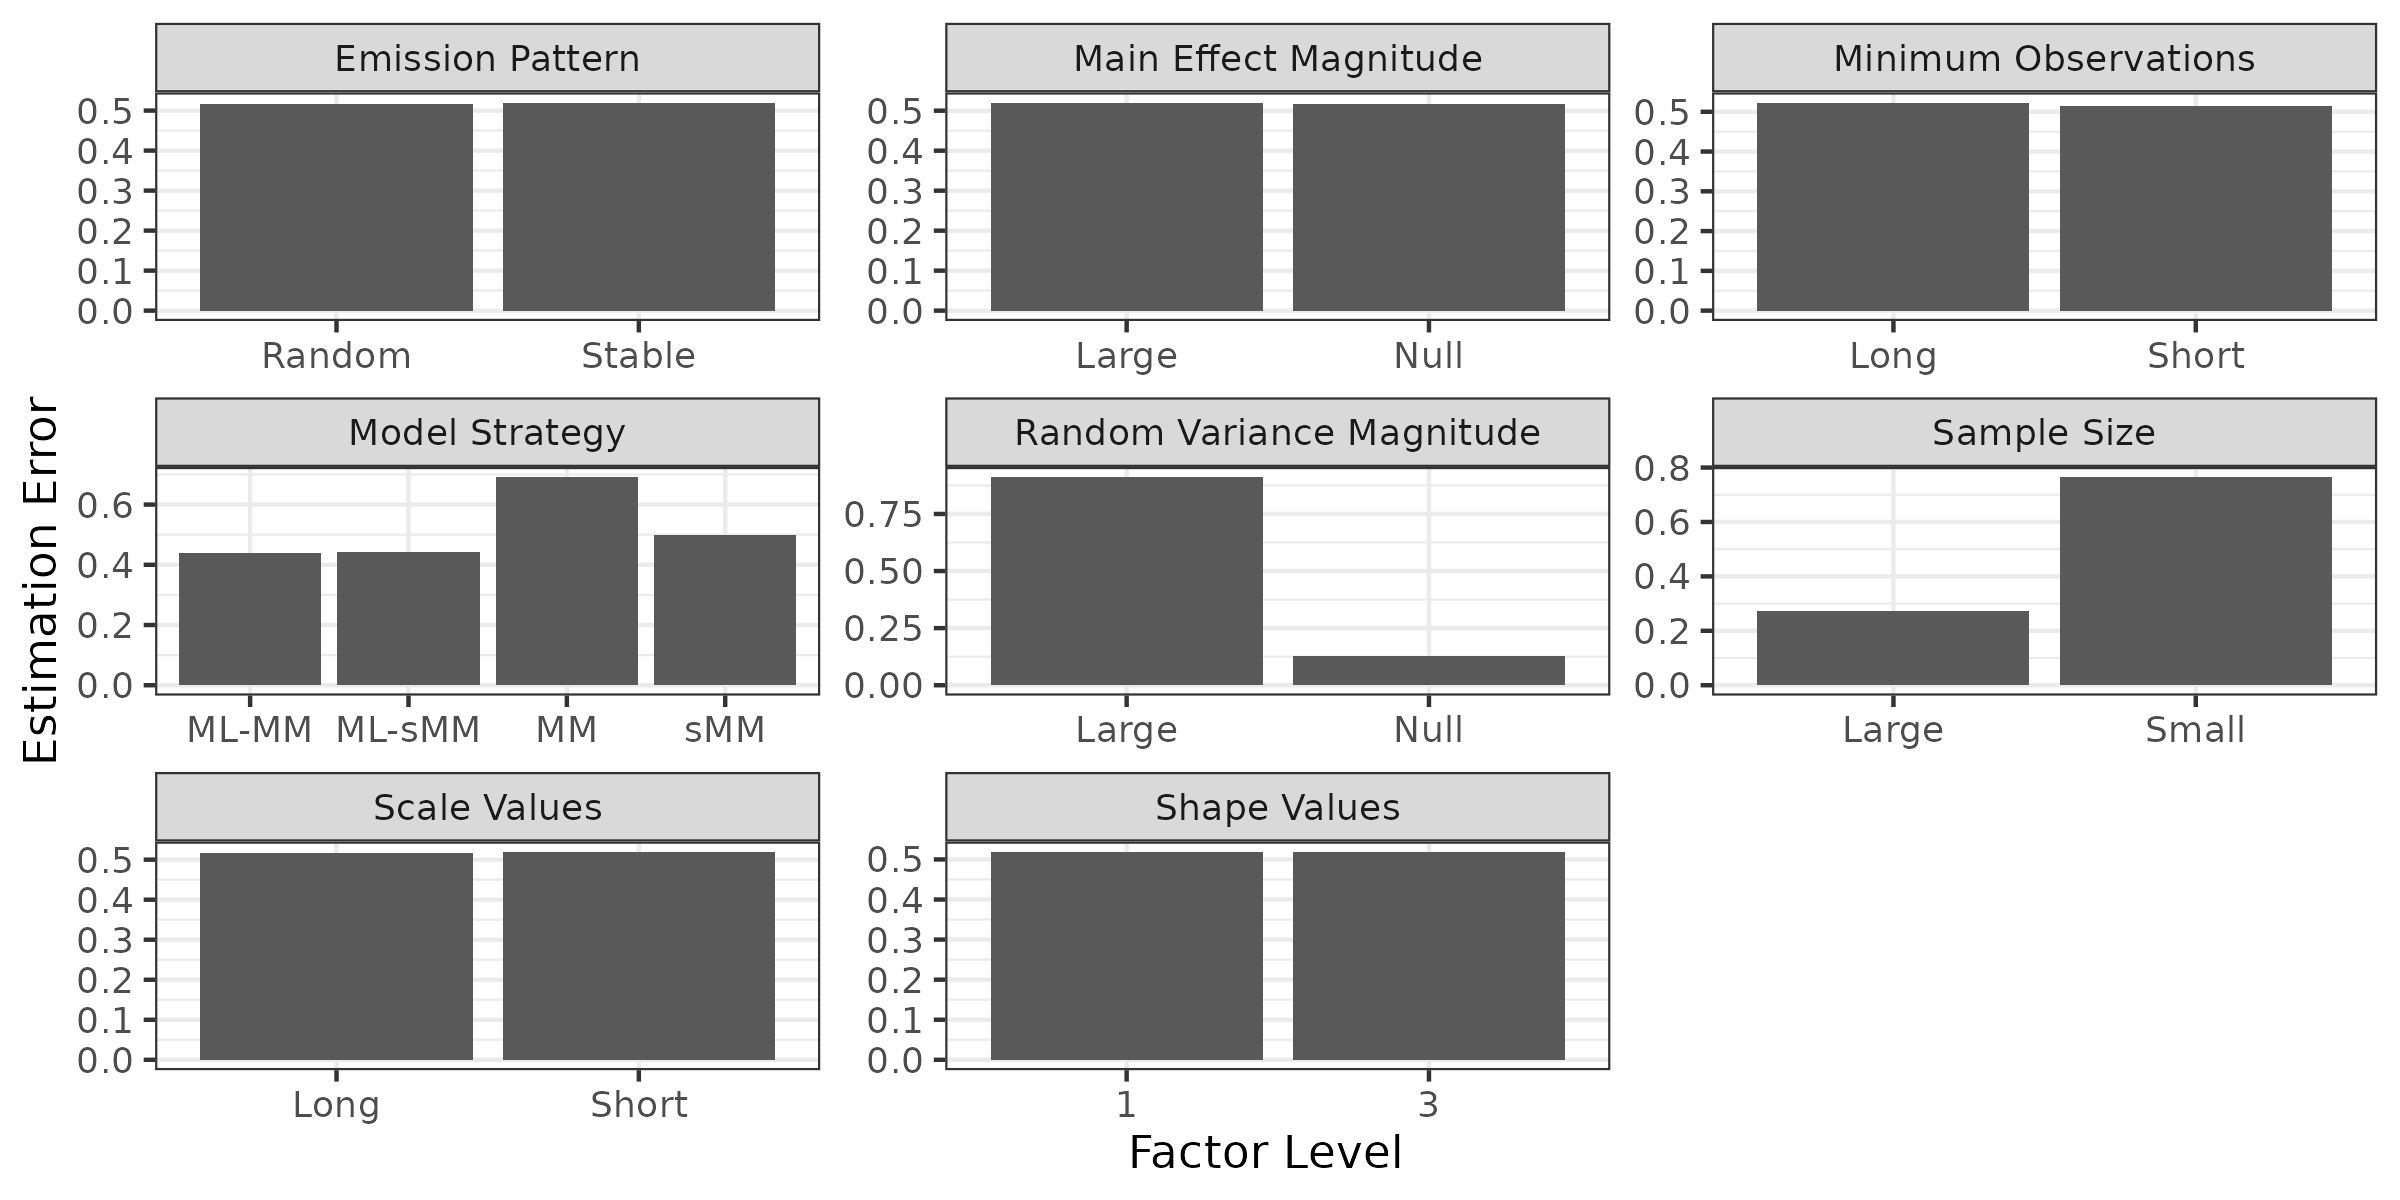
\includegraphics{figures/anova1MainEffect.png}
\end{frame}

\begin{frame}{Results question 1}
\phantomsection\label{results-question-1-2}
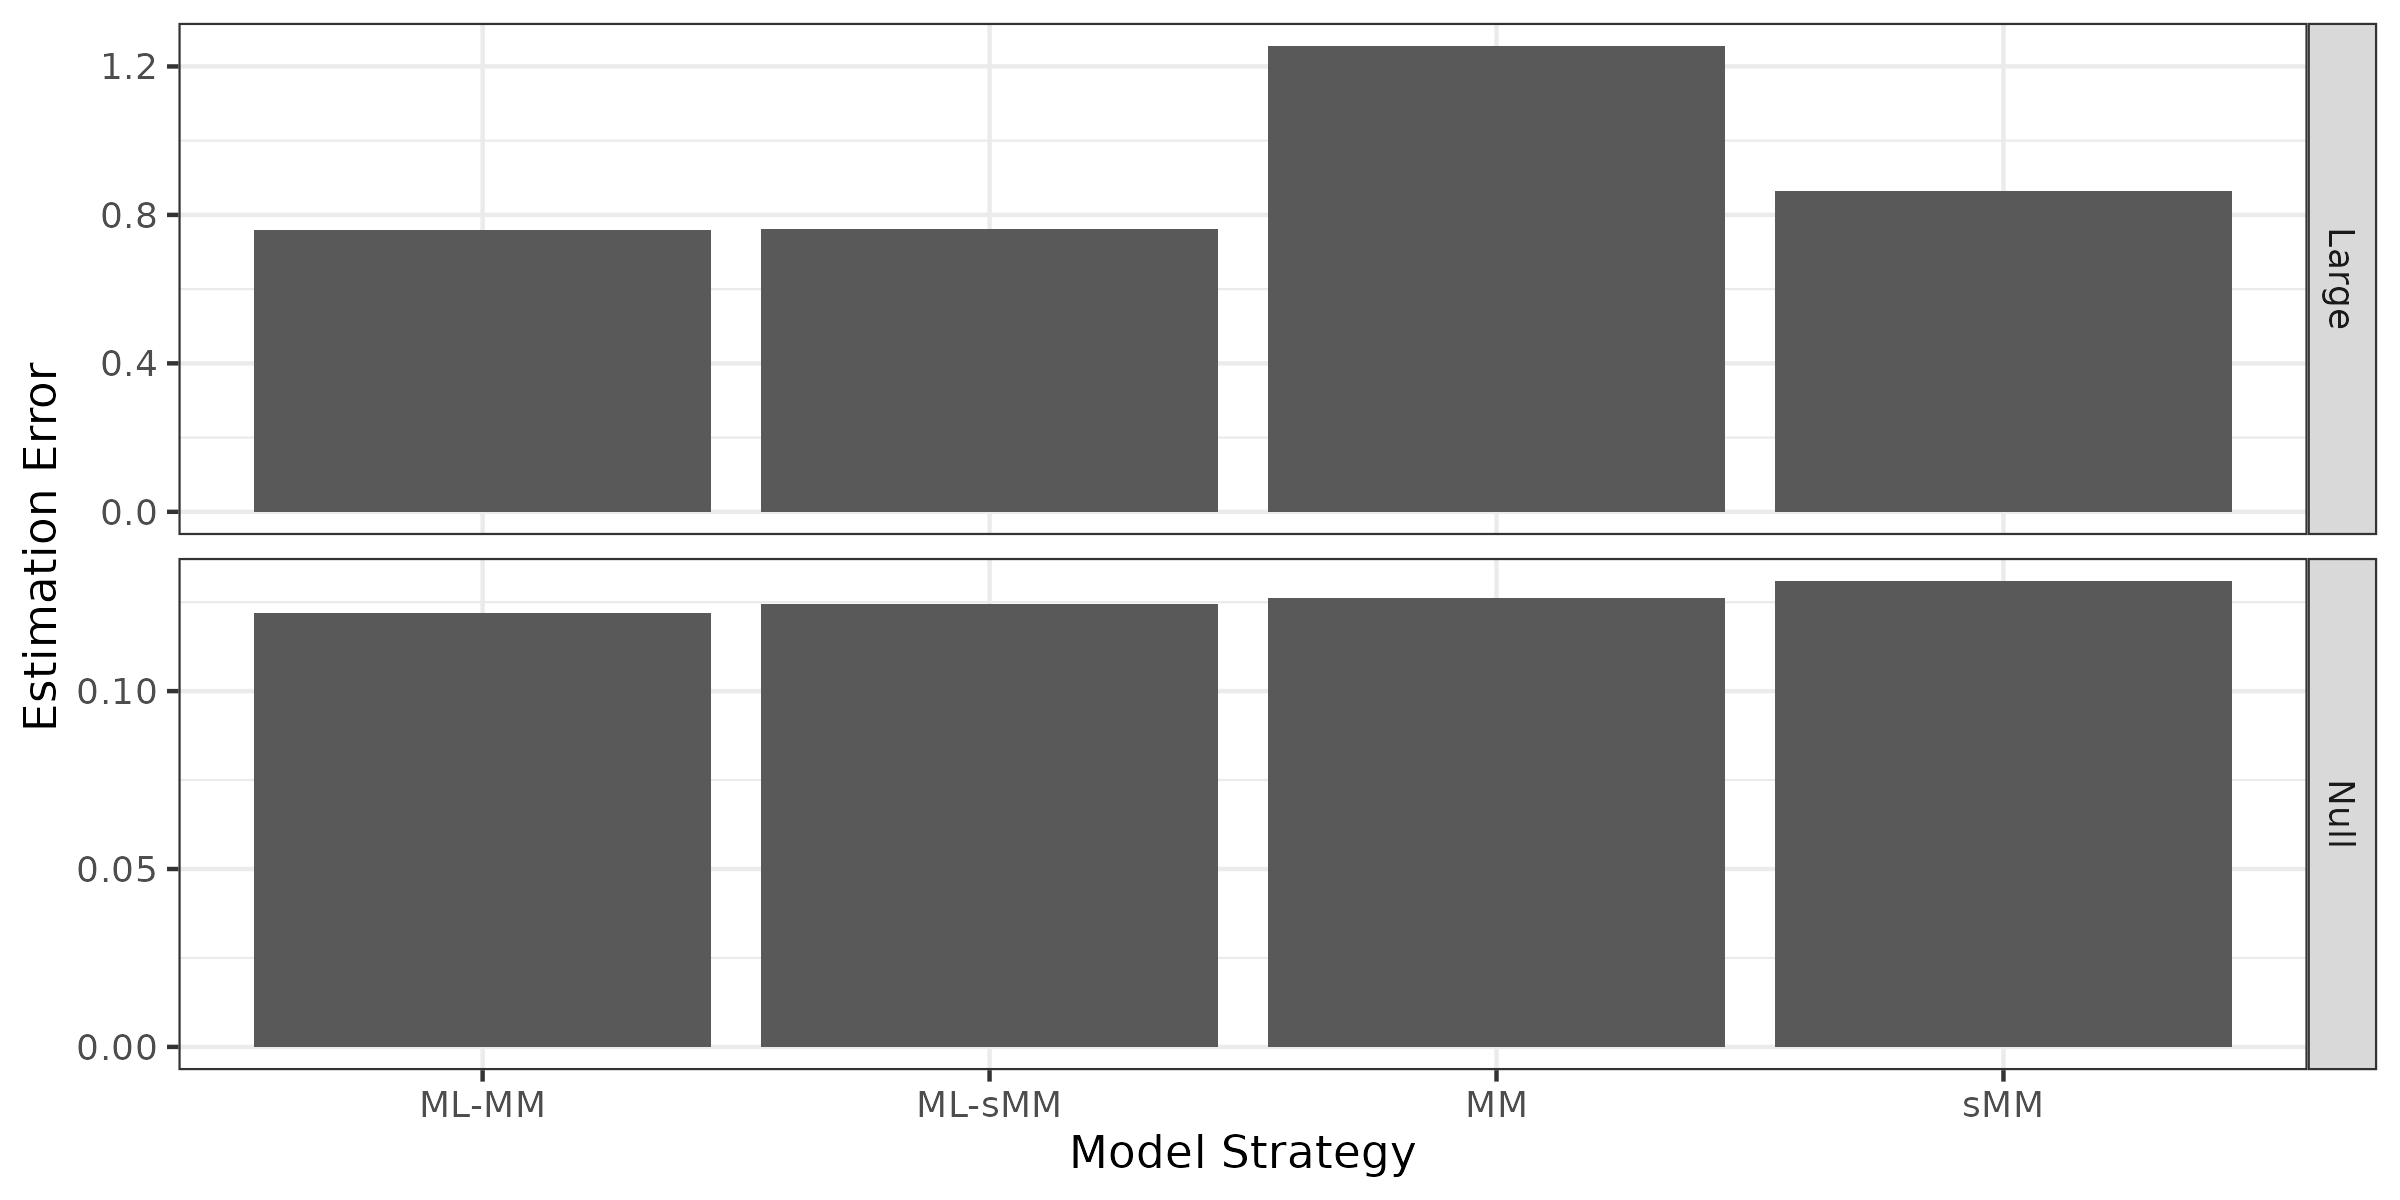
\includegraphics{figures/anova1TwoWay1.png}
\end{frame}

\begin{frame}{Results question 2}
\phantomsection\label{results-question-2}
\begin{enumerate}
\tightlist
\item
  Q2 examines the difference between the estimated and true shape
  parameter
\end{enumerate}

\begin{table}
    \centering
    \begin{tabular}{cc}
        Parameter & \(\eta^2\)\\
        Shape Parameter & .84 \\
        Model Strategy & .07 \\
        Magnitude of Random Variance & .02 \\
        Shape Parameter: Model Strategy & .04 \\
        Magnitude of Random Variance: Model Strategy & .03 \\
    \end{tabular}
\end{table}
\end{frame}

\begin{frame}{Results question 2}
\phantomsection\label{results-question-2-1}
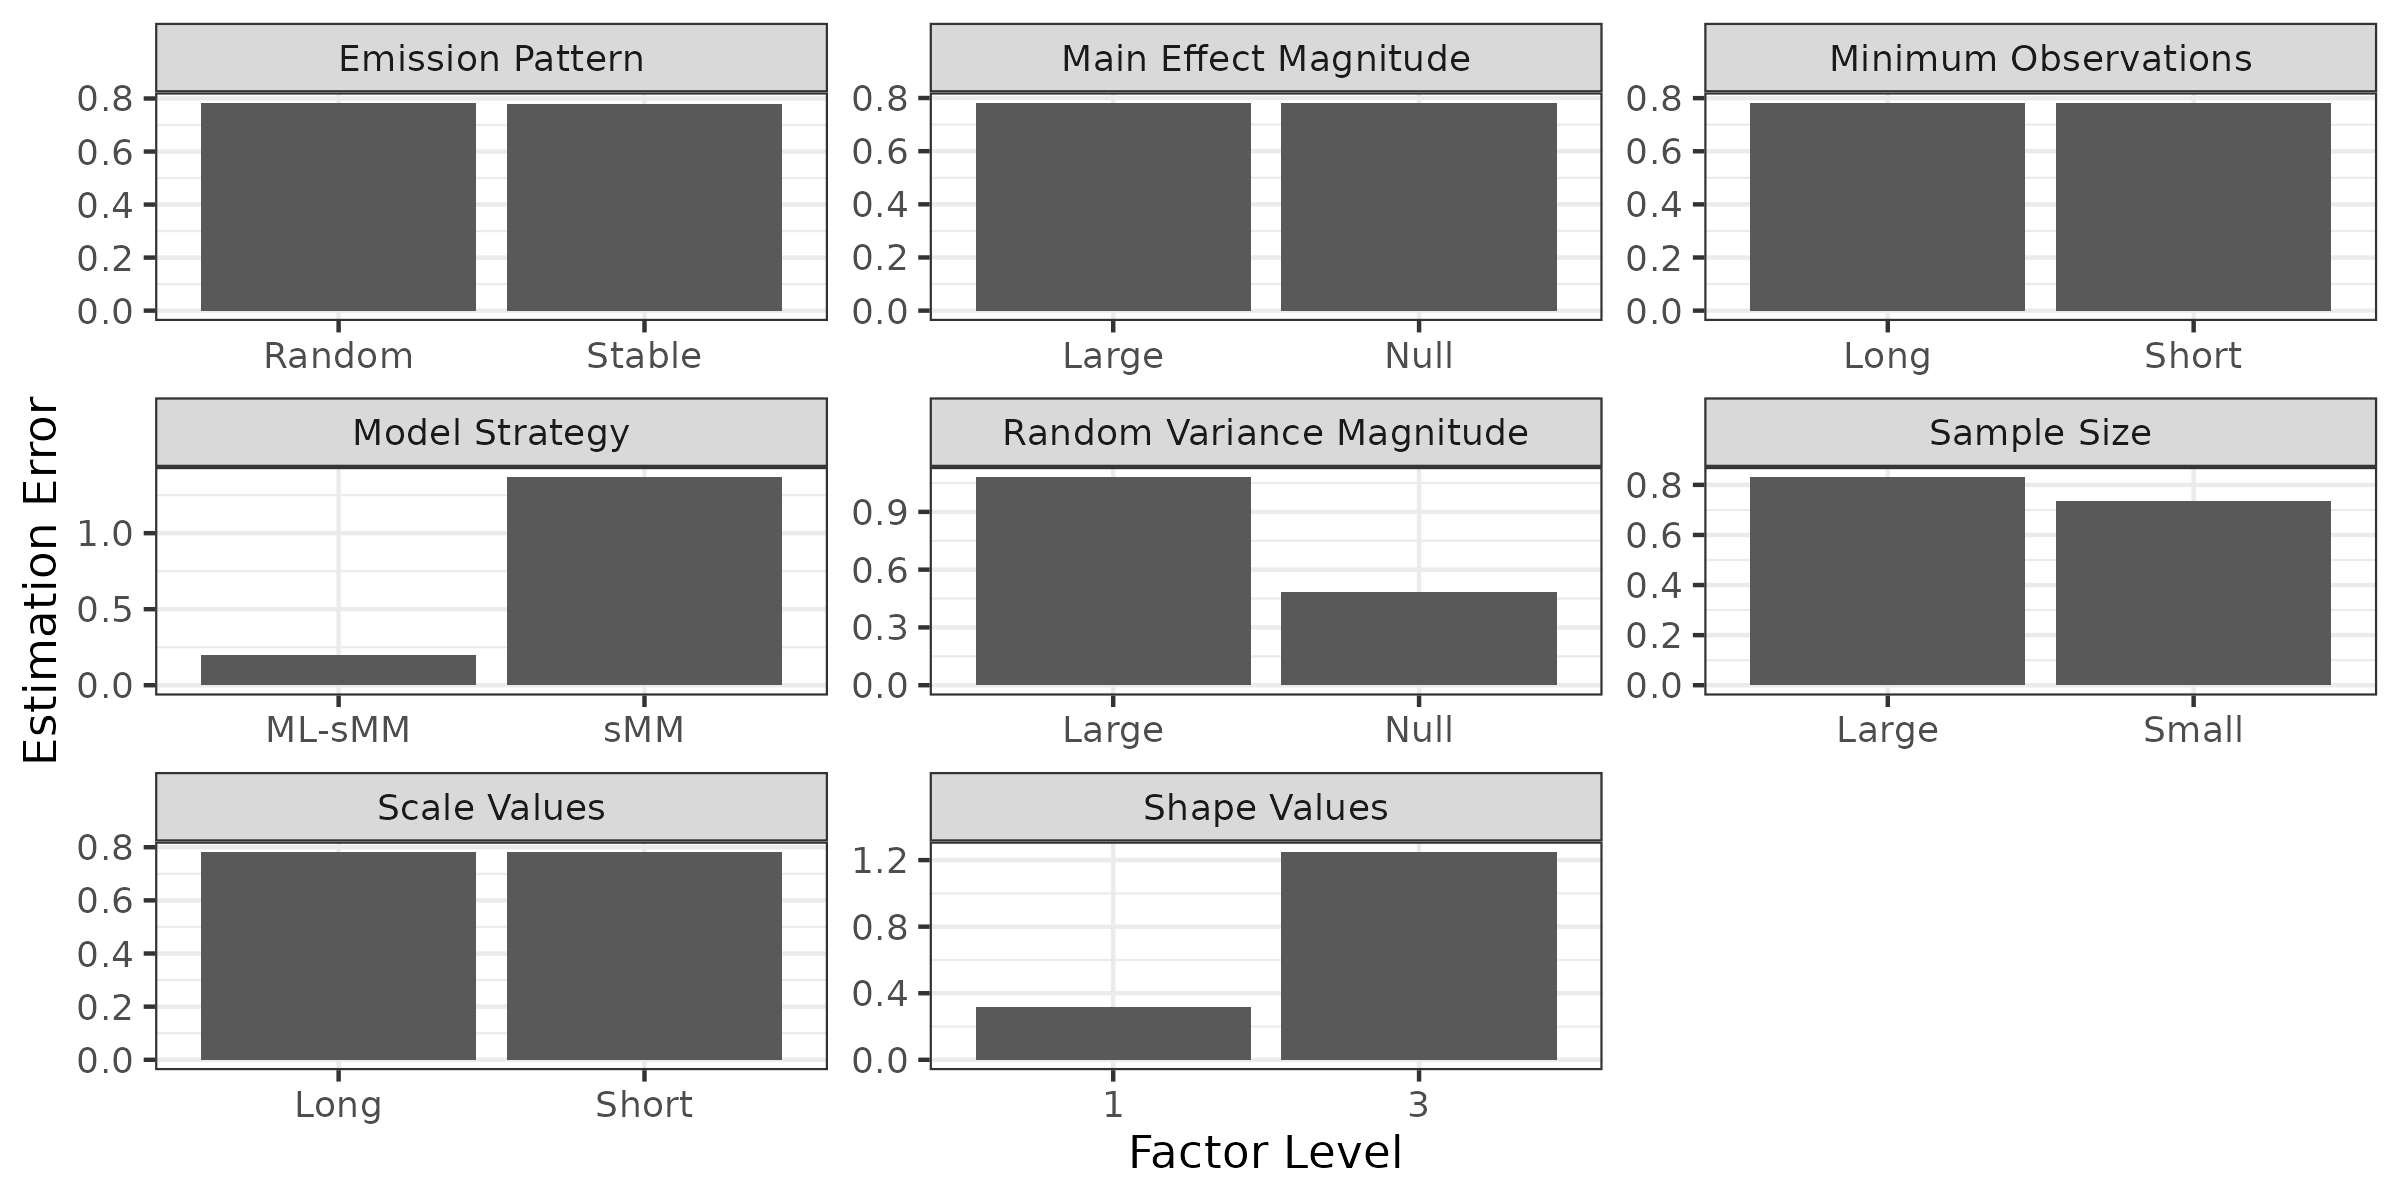
\includegraphics{figures/anova2MainEffect.png}
\end{frame}

\begin{frame}{Results question 2}
\phantomsection\label{results-question-2-2}
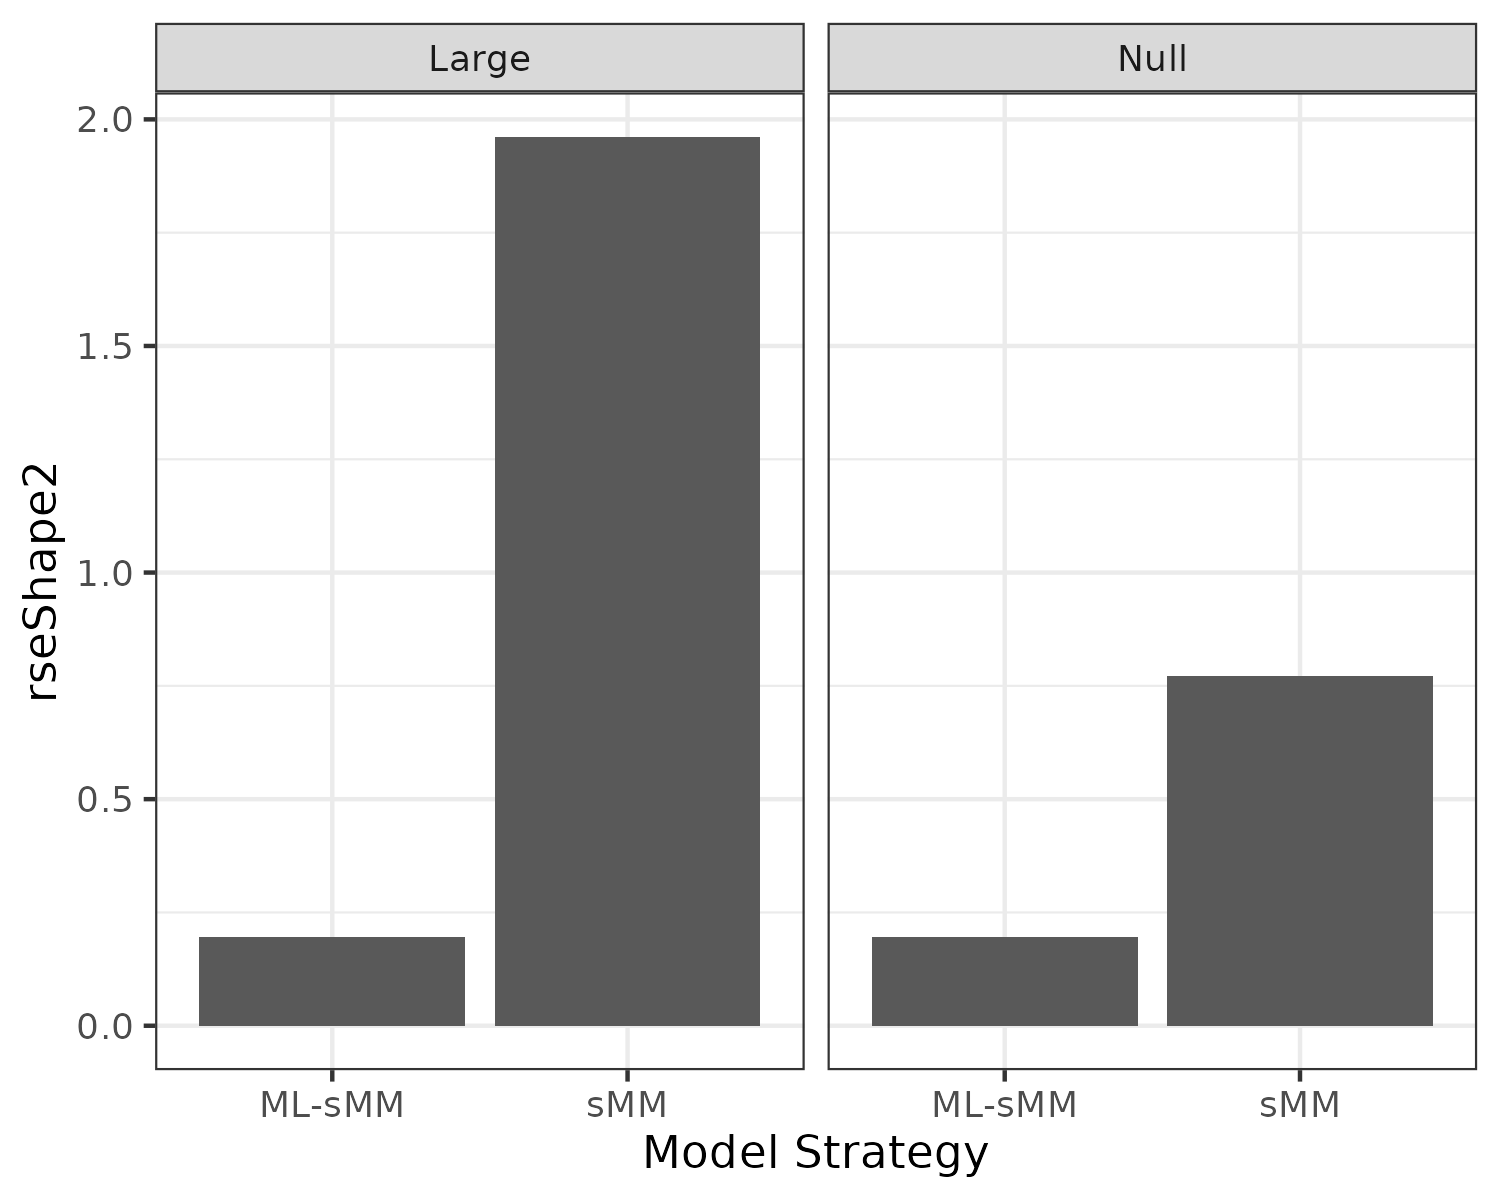
\includegraphics[width=\textwidth,height=2.70833in]{figures/anova2TwoWay1.png}
\end{frame}

\begin{frame}{Results question 3}
\phantomsection\label{results-question-3}
\begin{enumerate}
\tightlist
\item
  Q3 examines relationships between shape error and criterion variable
  error
\end{enumerate}

\begin{table}
    \centering
    \begin{tabular}{cc}
        Parameter & \(\eta^2\) \\
        Shape Error & .12 \\
        Shape Error:Shape Value & .04 \\
        Shape Error:Sample Size & .02\\
        Shape Error:Model Strategy & .01\\
        Shape Error:Shape Value:Sample Size & .01\\
    \end{tabular}
\end{table}
\end{frame}

\begin{frame}{Results question 3}
\phantomsection\label{results-question-3-1}
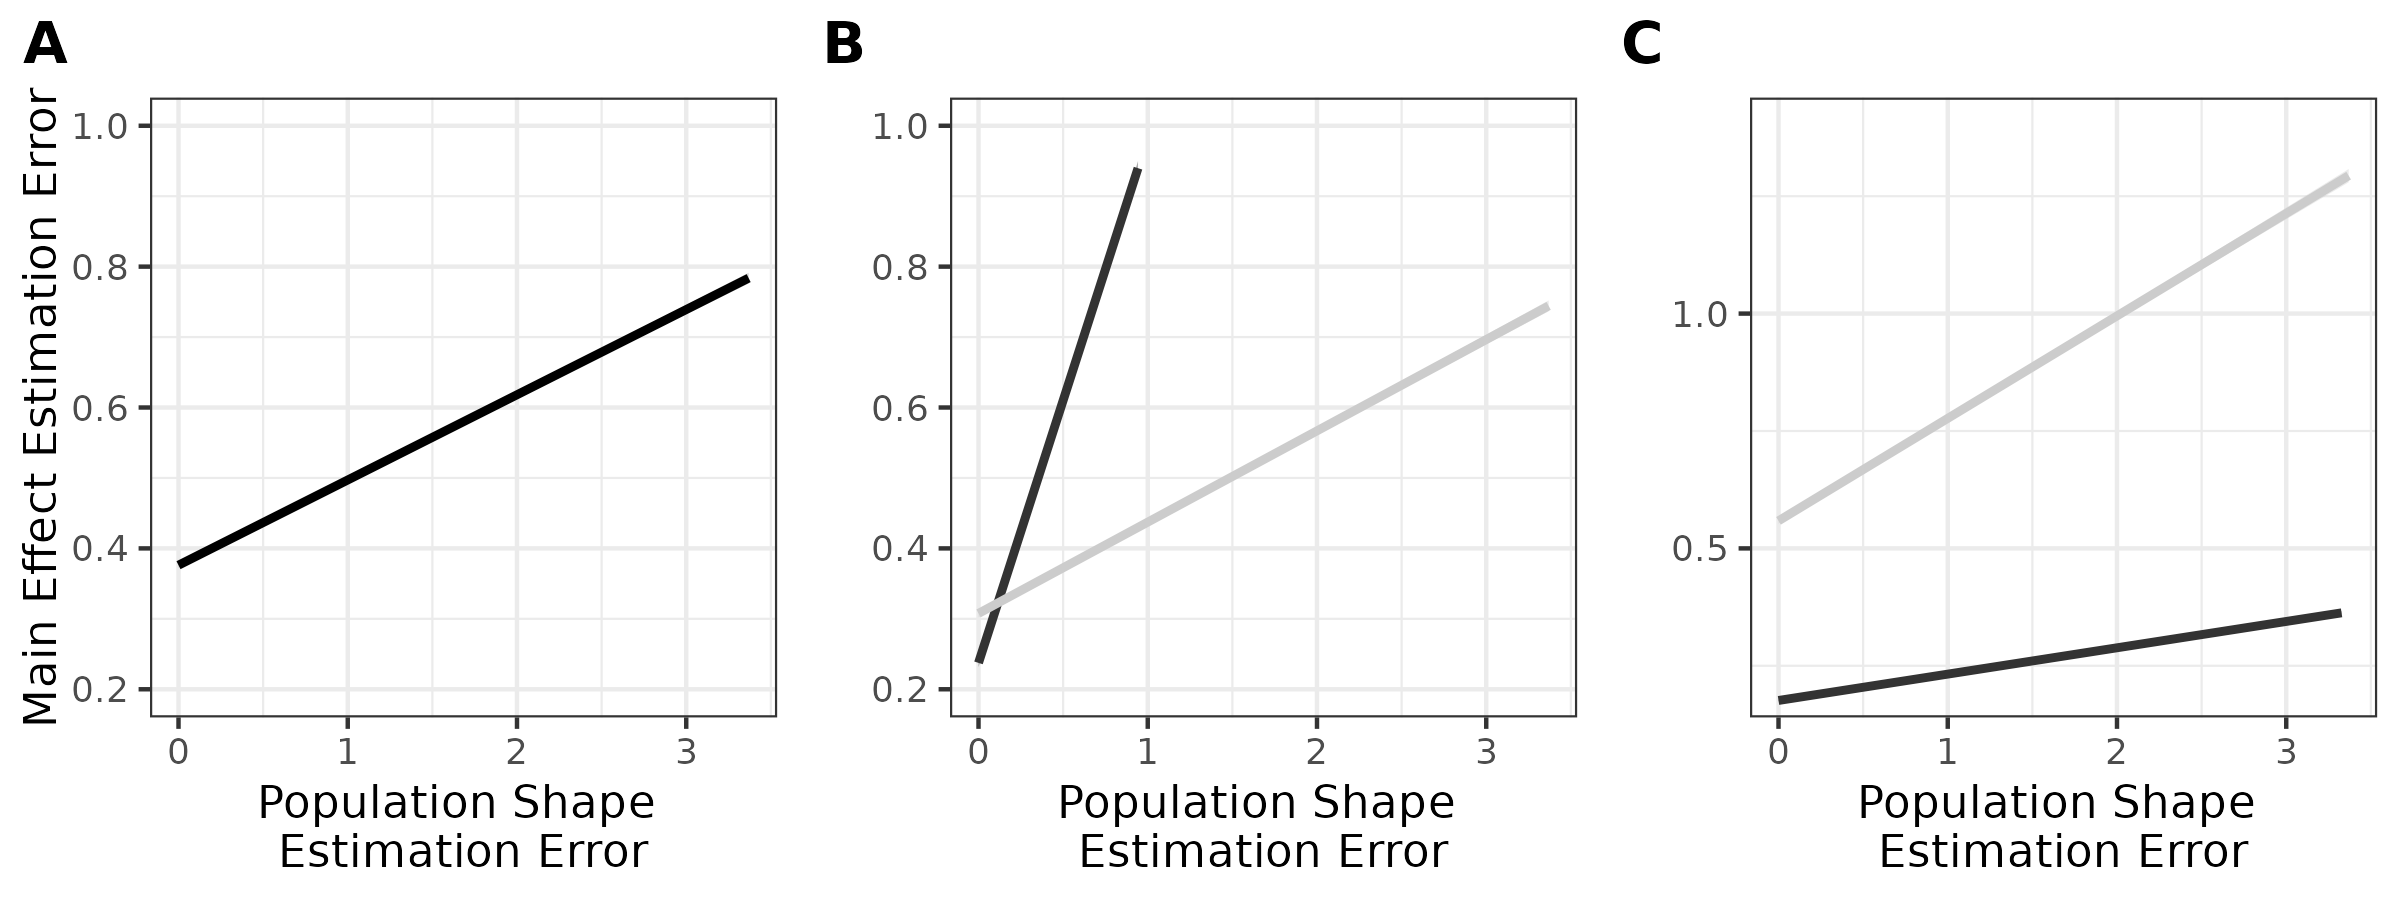
\includegraphics{figures/shapeEstimationError.png}
\end{frame}

\begin{frame}{Results question 4}
\phantomsection\label{results-question-4}
\begin{longtable}[]{@{}lll@{}}
\toprule\noalign{}
Parameters & Estimate & OR \\
\midrule\noalign{}
\endhead
Large Sample Size & 0.70 & 2.01 \\
Long Minimum Observation & -0.26 & 0.77 \\
Random Emission Pattern & 0.00 & 1.00 \\
Long Scale Values & 0.01 & 1.01 \\
Weibull Shape Parameter & -0.20 & 0.81 \\
Large Main Effect & -1.67 & 0.19 \\
Large Random Variance & -0.65 & 0.52 \\
ML-sMM & 0.56 & 1.75 \\
MM & -0.16 & 0.85 \\
ML-MM & 0.57 & 1.77 \\
\bottomrule\noalign{}
\end{longtable}
\end{frame}

\begin{frame}{Results question 4}
\phantomsection\label{results-question-4-1}
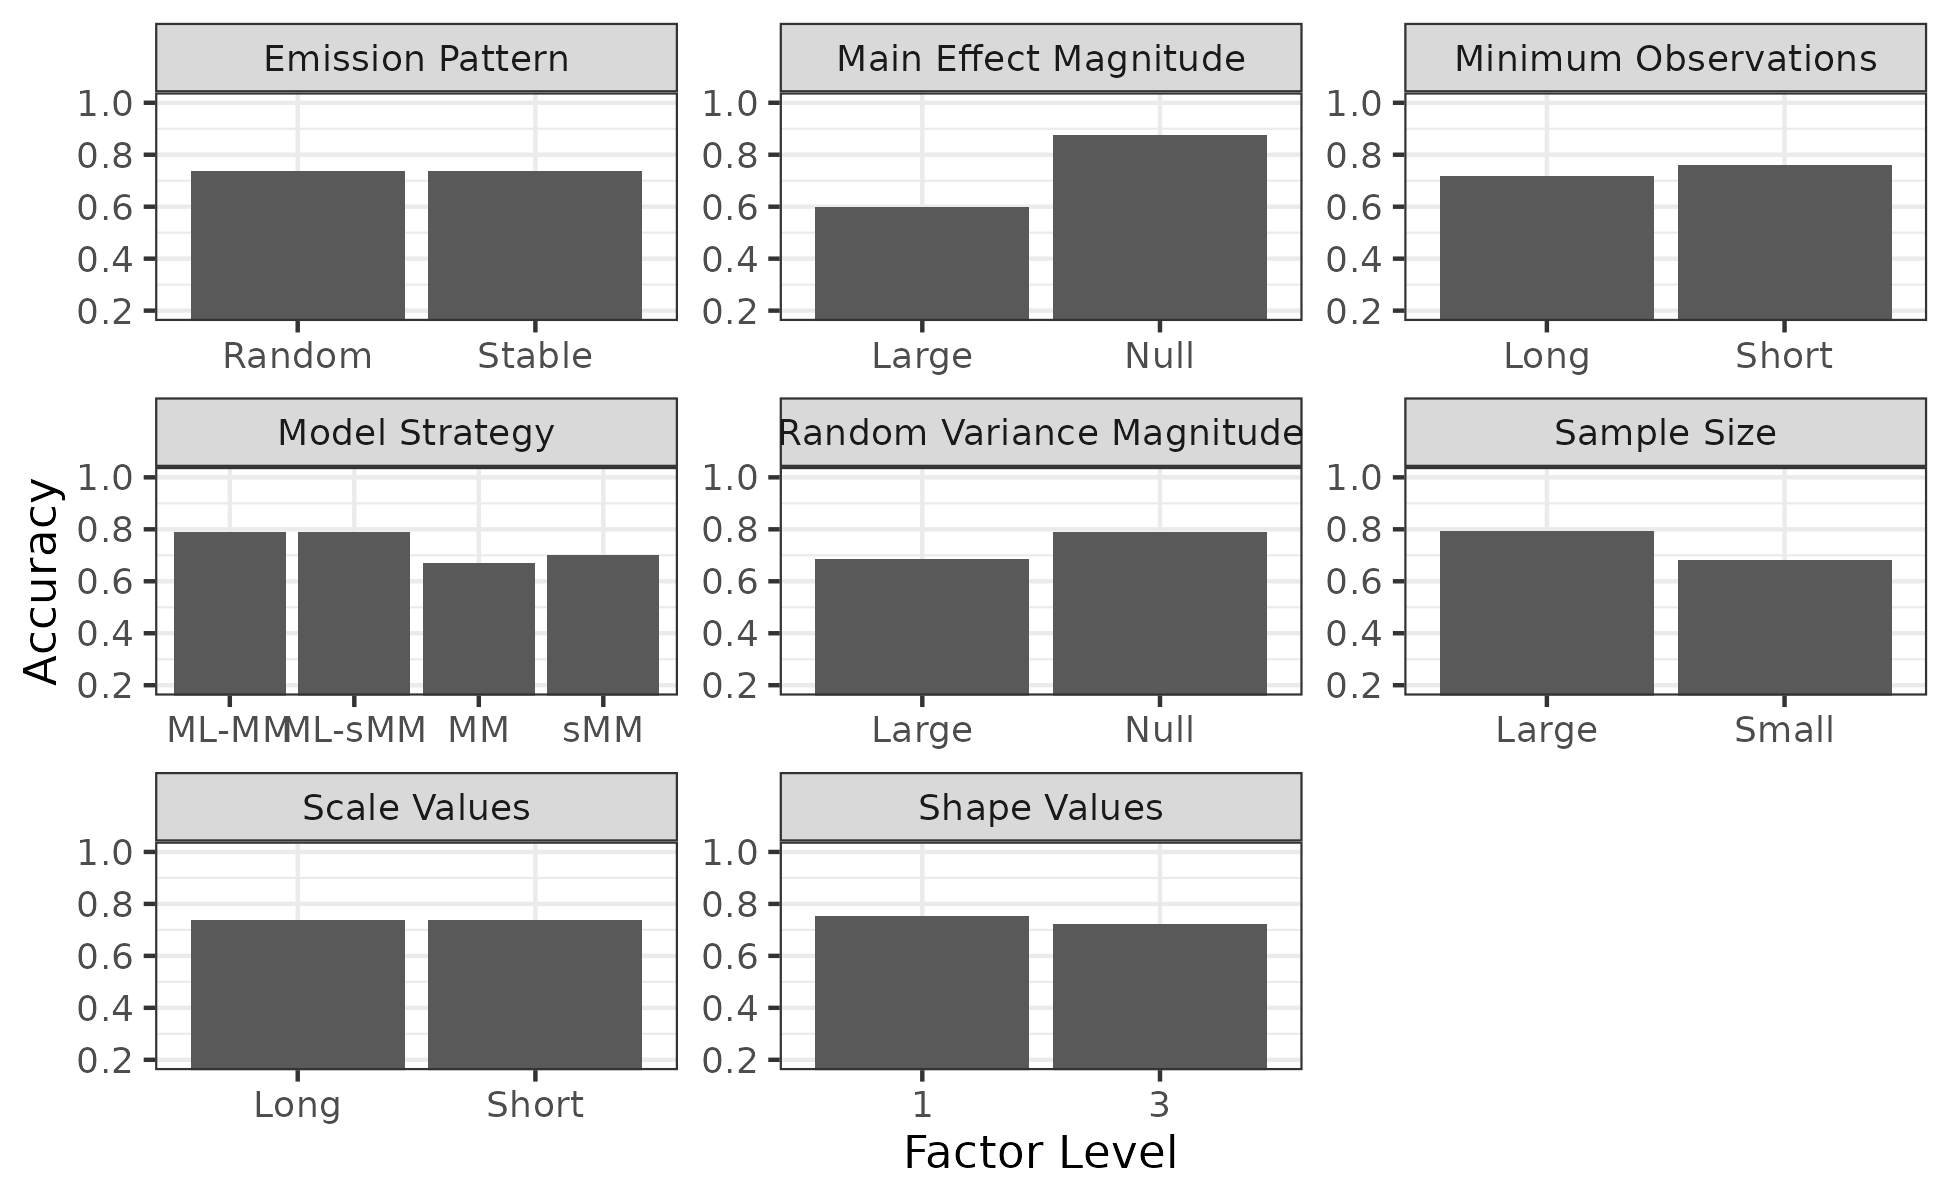
\includegraphics{figures/glm1MainEffect.png}
\end{frame}

\begin{frame}{Results question 4}
\phantomsection\label{results-question-4-2}
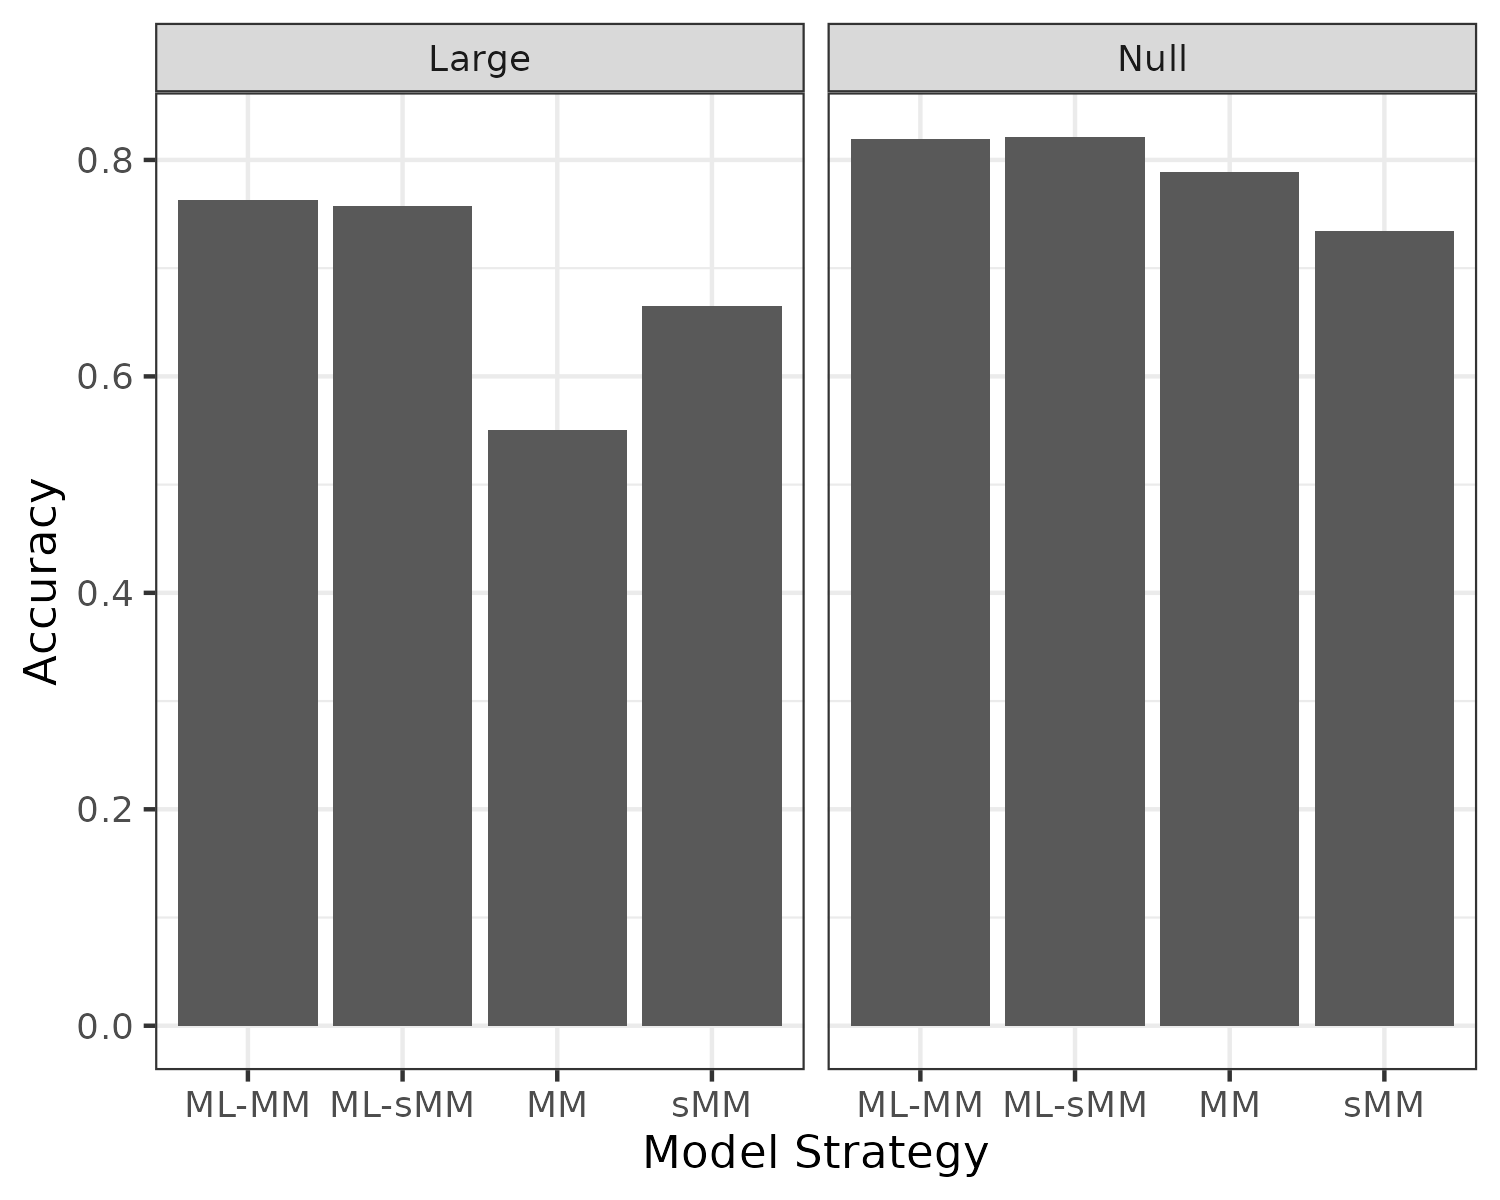
\includegraphics[width=\textwidth,height=2.60417in]{figures/glm1TwoWay1.png}
\end{frame}

\begin{frame}{Simulation summary}
\phantomsection\label{simulation-summary}
\begin{enumerate}
\item
  This simulation study has showcased the resilience of multilevel
  semi-Markov models
\item
  Question 1 detailed how the multilevel models had lower criterion
  variable estimation error compared to the fixed effect alternatives;
  additionally, a two-way interaction displayed how the MM had the
  greatest error when random variance existed
\item
  Question 2 detailed how the multilevel Weibull model performed better
  at recovering the true shape parameter
\item
  Question 3 detailed how mismatch between the estimated shape and the
  true shape parameter increases criterion variable error
\item
  Question 4 detailed how the multilevel models were much better at
  covering the true location of the criterion variable compared to the
  fixed effect alternatives
\end{enumerate}
\end{frame}

\section{Empirical}\label{empirical}

\begin{frame}{Introduction}
\phantomsection\label{introduction}
\begin{enumerate}
\tightlist
\item
  Parent child interaction therapy (PCIT) is a form of therapy that
  seeks to improve the relationship between a caregiver and their child
  (Eyberg 1988)
\item
  It is typically performed in a laboratory setting where a therapist
  can observe interactions between a caregiver and their child, and the
  caregiver is receiving instructions from the therapist with a bug in
  their ear
\item
  The underlying motivation is to increase PRIDE and decrease DON'T
  actions

  \begin{enumerate}
  \tightlist
  \item
    PRIDE skills include Behavior descriptions, Praise, Reflection,
    \textbf{Compliable commands}
  \item
    \href{https://www.youtube.com/watch?v=bldyeAk2InM}{Video example}
  \item
    DON'T skills generally include negative talk and noncompliable
    commands
  \end{enumerate}
\item
  A primary motiviation for the development of PCIT was the reduction of
  externalizing behavior issues
\end{enumerate}
\end{frame}

\begin{frame}{PCIT}
\phantomsection\label{pcit}
\begin{enumerate}
\item
  The administration of PCIT follows a protocol where child-directed
  (CDI) sessions are administered followed by parent-directed sessions
  (PDI).

  \begin{enumerate}
  \tightlist
  \item
    CDI is focused on encouraging PRIDE skills, and providing the
    caregiver guidance to follow the child's lead in play sessions
  \item
    PDI is focused on instructing the parent for how to deliver high
    quality commands, and when the commands are not complied with,
    structured disciplinary practices:
    \href{https://youtu.be/CeVhVTAX9v0?t=219}{Time out example}
  \item
    Mastery of CDI is met when parent have displayed more than 10 PRIDE
    skills during a single play session
  \item
    Mastery of PDI is met when the parent delivers effective commands,
    rewards compliance with praise, and practices administers the
    timeout procedure when appropriate
  \end{enumerate}
\item
  The \textbf{Dyadic Parent Child Coding System (DPICs)} is one example
  of a task developed specifically for PCIT (Nelson and Olsen 2018).
\end{enumerate}
\end{frame}

\begin{frame}{The DPICs design}
\phantomsection\label{the-dpics-design}
\begin{columns}[T]
\begin{column}{0.5\textwidth}
The DPICs is a laboratory administered task which examines the
interaction quality between a caregiver-child dyad

caregiver verbal actions are coded into one of three categories during
three 5-minute sessions:

\begin{enumerate}
\item
  Child-led play
\item
  Parent-led play
\item
  \textbf{Clean-up task}
\end{enumerate}

The clean-up task requires the caregiver to instruct the child to put
toys back into their boxes without assistance from the caregiver.
\end{column}

\begin{column}{0.5\textwidth}
\includegraphics{figures/dpicsTimeSeries.png}
\end{column}
\end{columns}
\end{frame}

\begin{frame}{Examining the influence of the child's behavior on
caregiver actions}
\phantomsection\label{examining-the-influence-of-the-childs-behavior-on-caregiver-actions}
\begin{enumerate}
\tightlist
\item
  Children's noncompliance with parental requests represents the most
  common externalizing problem for which parents seek child mental
  health services (Owen, Slep, and Heyman 2012; Kalb and Loeber 2003;
  Chamberlain and Smith 2003).
\item
  Parents who report greater hostility and elevated child externalizing
  problems are 35\% more likely to engage with their children when
  noncompliance is observed (Lunkenheimer et al. 2016)
\item
  Better self-regulation supports parents in refraining from reactive
  negative parenting (Geeraerts et al. 2021); conversely, poorly
  regulated parents are more inclined toward harsh and controlling
  parenting practices and negative affect toward children who generally
  show more hard-to-manage behavior (Deater-Deckard et al. 2012)
\end{enumerate}
\end{frame}

\begin{frame}{Previous time-series DPICs analyses}
\phantomsection\label{previous-time-series-dpics-analyses}
\begin{enumerate}
\tightlist
\item
  The analysis of DPICs data is typically performed by tallying the
  total number of each verbal expression

  \begin{enumerate}
  \tightlist
  \item
    For example CDI mastery is assessed by tallying total number of
    PRIDE actions
  \end{enumerate}
\item
  A literature review which examined analyses specific to the DPICs
  clean-up task revealed two studies similar to the scope of this
  analysis:

  \begin{enumerate}
  \tightlist
  \item
    Somers et al., 2023
  \item
    Lunkenheimer et al., 2017
  \end{enumerate}
\end{enumerate}
\end{frame}

\begin{frame}{Somers et al., 2023}
\phantomsection\label{somers-et-al.-2023}
\begin{enumerate}
\item
  In this study researchers examine the interrelations between parent's
  behaviors and child compliance
\item
  A multilevel dynamic factor analysis was used to model relationships
  between parent's and child's behaviors in 10-second epochs
\item
  Parent and child behaviors were coded as binary variables within every
  epoch
\end{enumerate}

\includegraphics[width=3.125in,height=\textheight]{images/clipboard-3731853544.png}
\end{frame}

\begin{frame}{Somers et al., cont.}
\phantomsection\label{somers-et-al.-cont.}
\includegraphics{images/clipboard-2206082127.png}
\end{frame}

\begin{frame}{Somers et al., cont.}
\phantomsection\label{somers-et-al.-cont.-1}
``This study suggests that parents' behavior precipitates the onset of
child noncompliance. Yet, specific parental antecedents of child
noncompliance differ depending on the context, highlighting ways parents
can adjust how they give commands and respond to child behavior that may
promote children's well-regulated, compliant behavior.'' (Somers et al.
2024)
\end{frame}

\begin{frame}{Lunkenheimer et al.,}
\phantomsection\label{lunkenheimer-et-al.}
\begin{enumerate}
\tightlist
\item
  This study examined positive, autonomy supportive behavior coupling
  related to changes in children's behavioral responses and coupling
  related to changes in mother's behavioral responses
\item
  Parents and children were coded for affect and goal-directed behavior
  on a second-by-second basis and codes were mutually exclusive; only
  the codes for goal-directed behavior were used for the present study.
\item
  A continuous-time hidden Markov model was used to examine dynamics
  across the behaviors
\end{enumerate}

\includegraphics[width=3.125in,height=\textheight]{images/Screenshot from 2024-06-03 14-12-42-01.png}
\end{frame}

\begin{frame}{Lunkenheimer et al., cont.}
\phantomsection\label{lunkenheimer-et-al.-cont.}
\begin{enumerate}
\item
  This study used transitions into and out of states 1,2, and 4 as the
  outcome variable, the results suggested:

  \begin{enumerate}
  \item
    For parents who endorse higher levels of harsh parenting, the child
    was less likely to make use of the mother's autonomy-supportive
    parenting practices and transition into autonomous behavior.
  \item
    For parents who endorse higher levels of harsh parenting when
    children displayed positive, autonomous behavior, the mother was
    less likely to transition into parenting behaviors that supported
    that autonomy.
  \end{enumerate}
\end{enumerate}
\end{frame}

\begin{frame}{Hypotheses}
\phantomsection\label{hypotheses}
\begin{enumerate}
\tightlist
\item
  PCIT will decrease the transition intensities into the DON'T state;
  and increase transition intensities into the PRIDE state
\item
  Child compliance will increase the transition intensity into the PRIDE
  state after the administration of PCIT
\end{enumerate}
\end{frame}

\begin{frame}{Methods}
\phantomsection\label{methods-1}
\begin{enumerate}
\item
  Pre- and post-PCIT DPICs data were acquired from 204 parent-child
  dyads using an intervention versus control RCT design.
\item
  The sample was drawn from consecutive family referrals received
  between April 2016 and June 2019 from the Department of Human
  Services-Child Welfare and Self-Sufficiency, and who consented to
  enroll in the study.
\end{enumerate}

\begin{longtable}[]{@{}lll@{}}
\toprule\noalign{}
Cohort & Pre & Post \\
\midrule\noalign{}
\endhead
Intervention & 115 & 87 \\
Control & 83 & 63 \\
\bottomrule\noalign{}
\end{longtable}
\end{frame}

\begin{frame}{Methods cont.}
\phantomsection\label{methods-cont.}
\begin{enumerate}
\tightlist
\item
  Verbal interactions form the parents were coded into one of three
  categories

  \begin{enumerate}
  \tightlist
  \item
    PRIDE: Compliable Commands, Behavior Description, Praise, Reflection
  \item
    Neutral: Neutral Talk, Questions
  \item
    DON'T: Negative Talk, Non-Compliable Commands
  \end{enumerate}
\end{enumerate}

\includegraphics[width=\textwidth,height=1.45833in]{figures/dpicsTimeSeries.png}
\end{frame}

\begin{frame}{Methods cont.}
\phantomsection\label{methods-cont.-1}
Multilevel Weibull models were estimated to examine timing between
transitions (n=23,862), and how pre- and post-PCIT influences these
transition intensities

Models took the following form:
sojournTime\textasciitilde(transType+wave+PCIT)\^{}3

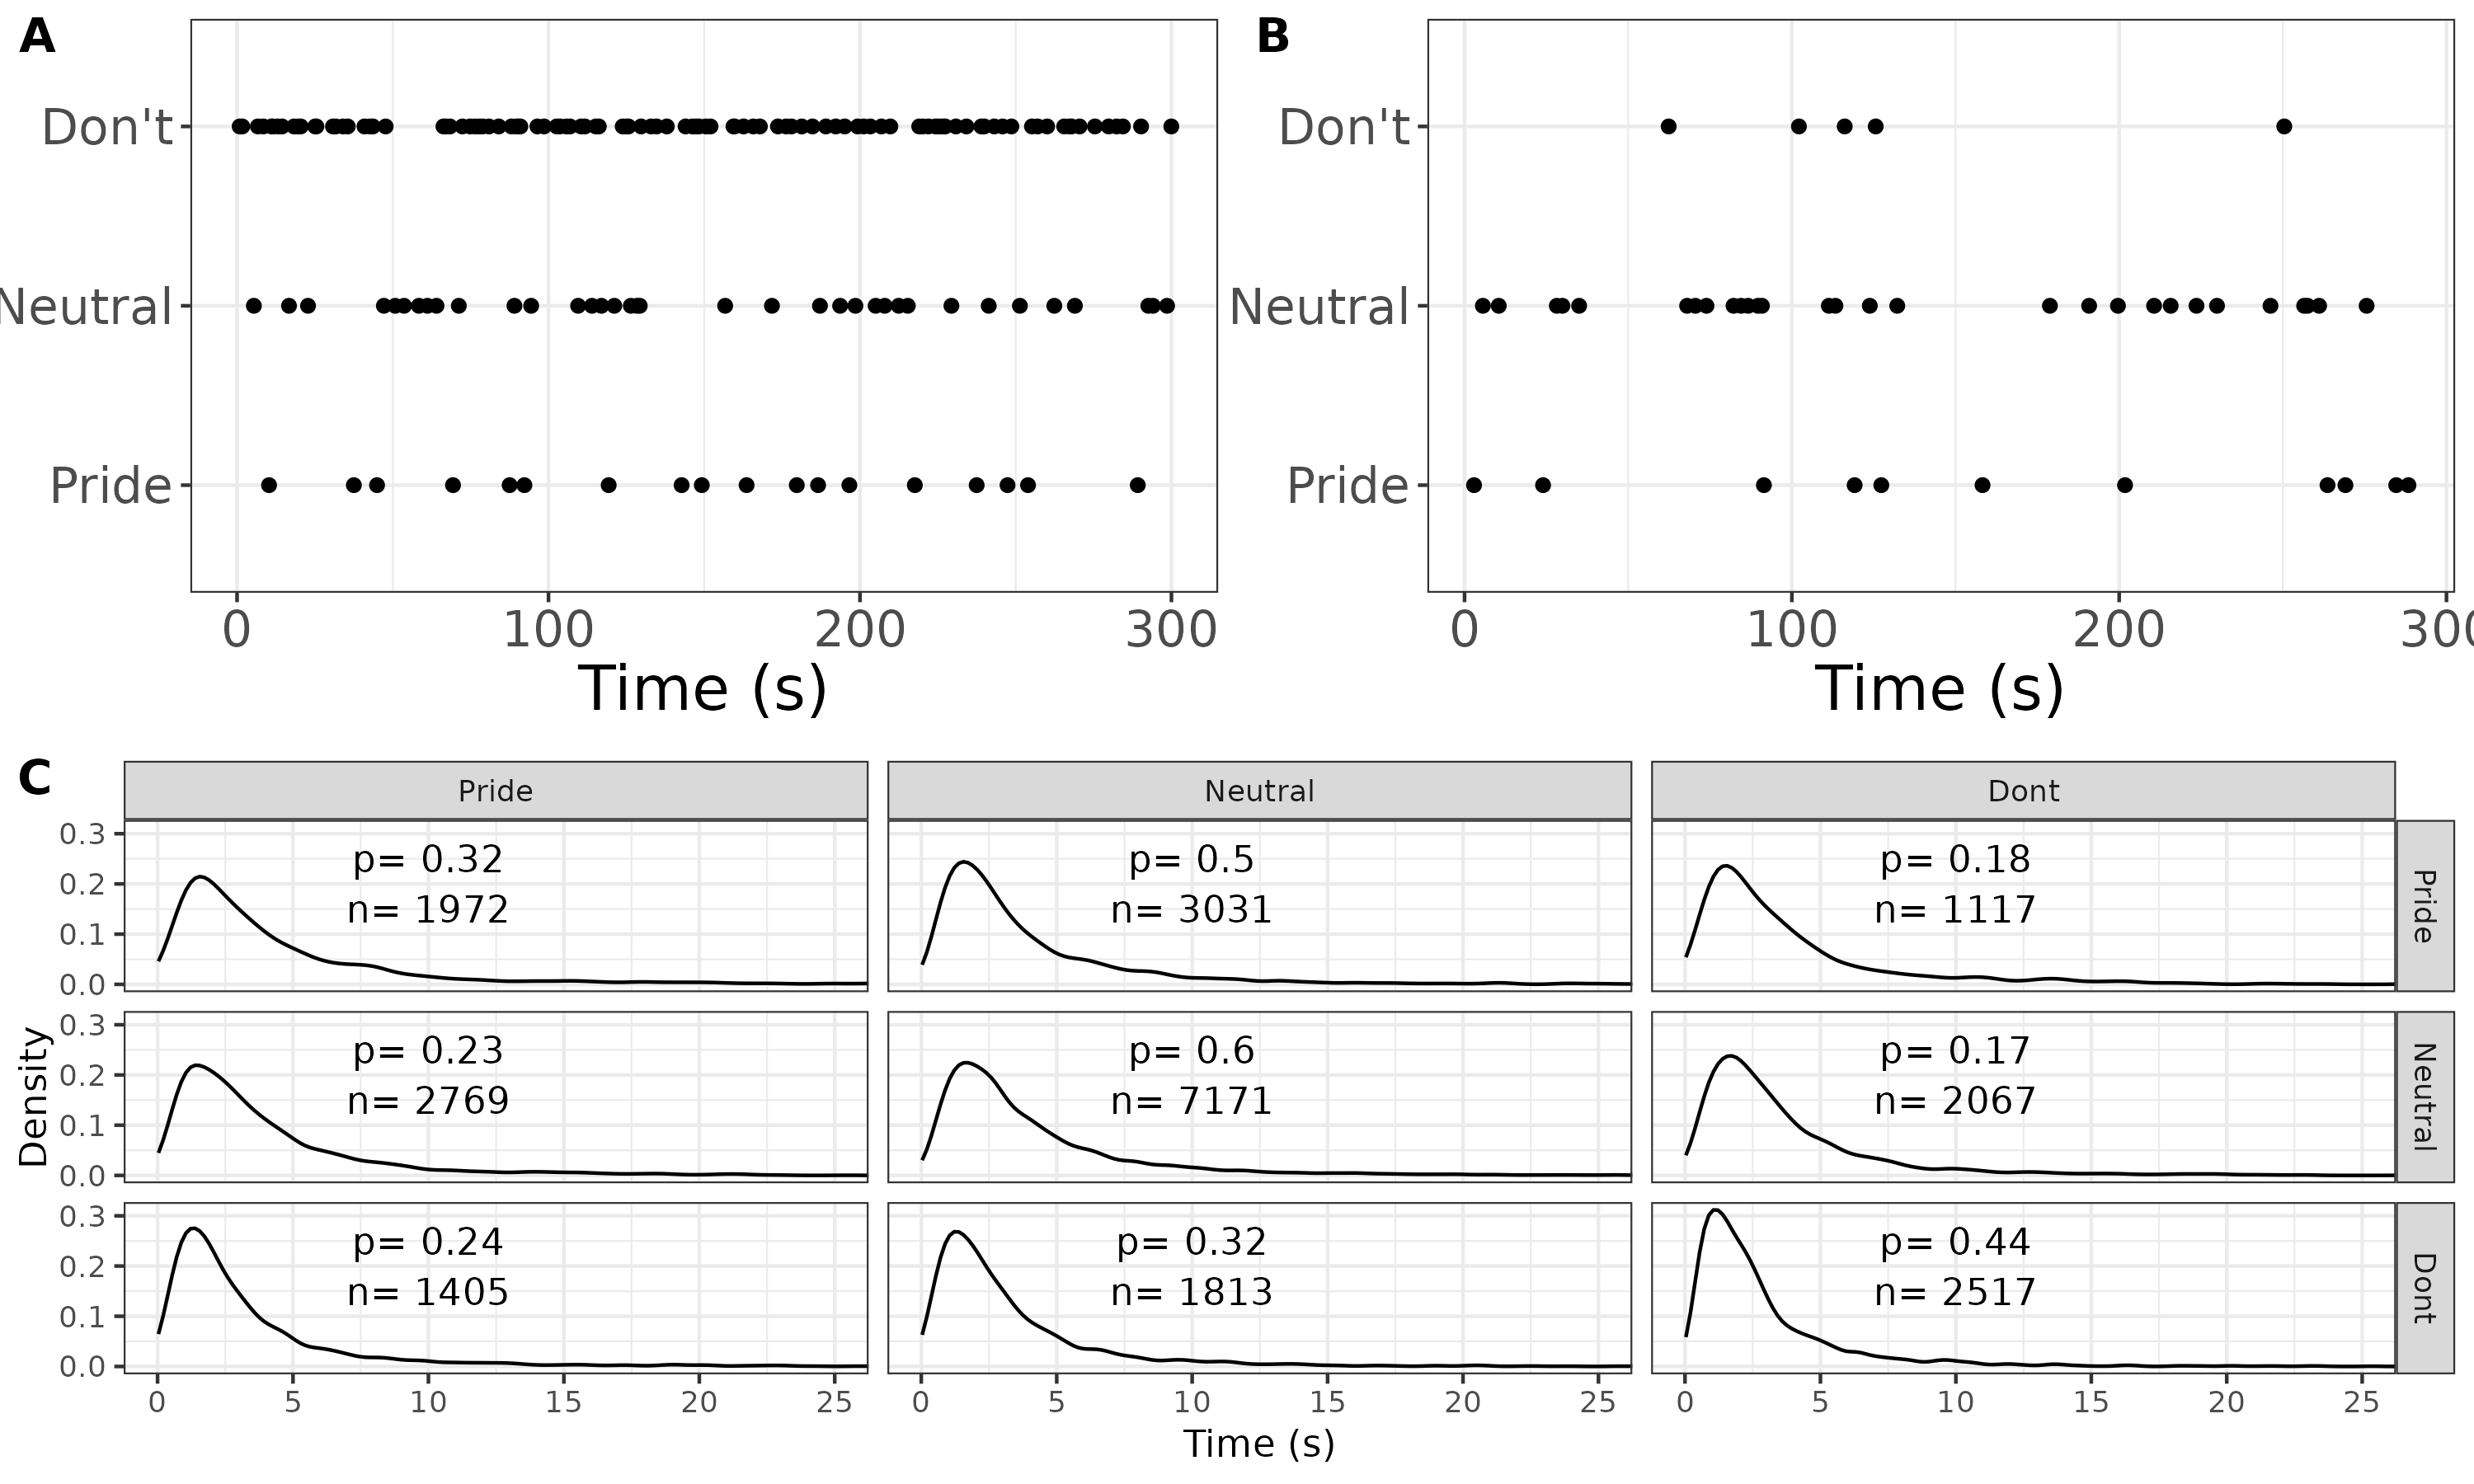
\includegraphics[width=2.5in,height=\textheight]{figures/CLUPTimeSeries.png}
\end{frame}

\begin{frame}{Methods cont.}
\phantomsection\label{methods-cont.-2}
The influence of child compliance on parental behaviors was examined in
a separate model

This model examined the sojourn times following the delivery of any
compliable command

The model takes the following form: sojournTime \textasciitilde{}
(nextState+wave+PCIT+compliance)\^{}4

All models were estimated in a Bayesian framework, 10,000 permutations,
2,000 warm-up, thinning of 10, 6 chains were run, samples were generated
using the NUTS algorithm implemented in STAN
\end{frame}

\begin{frame}{Results}
\phantomsection\label{results}
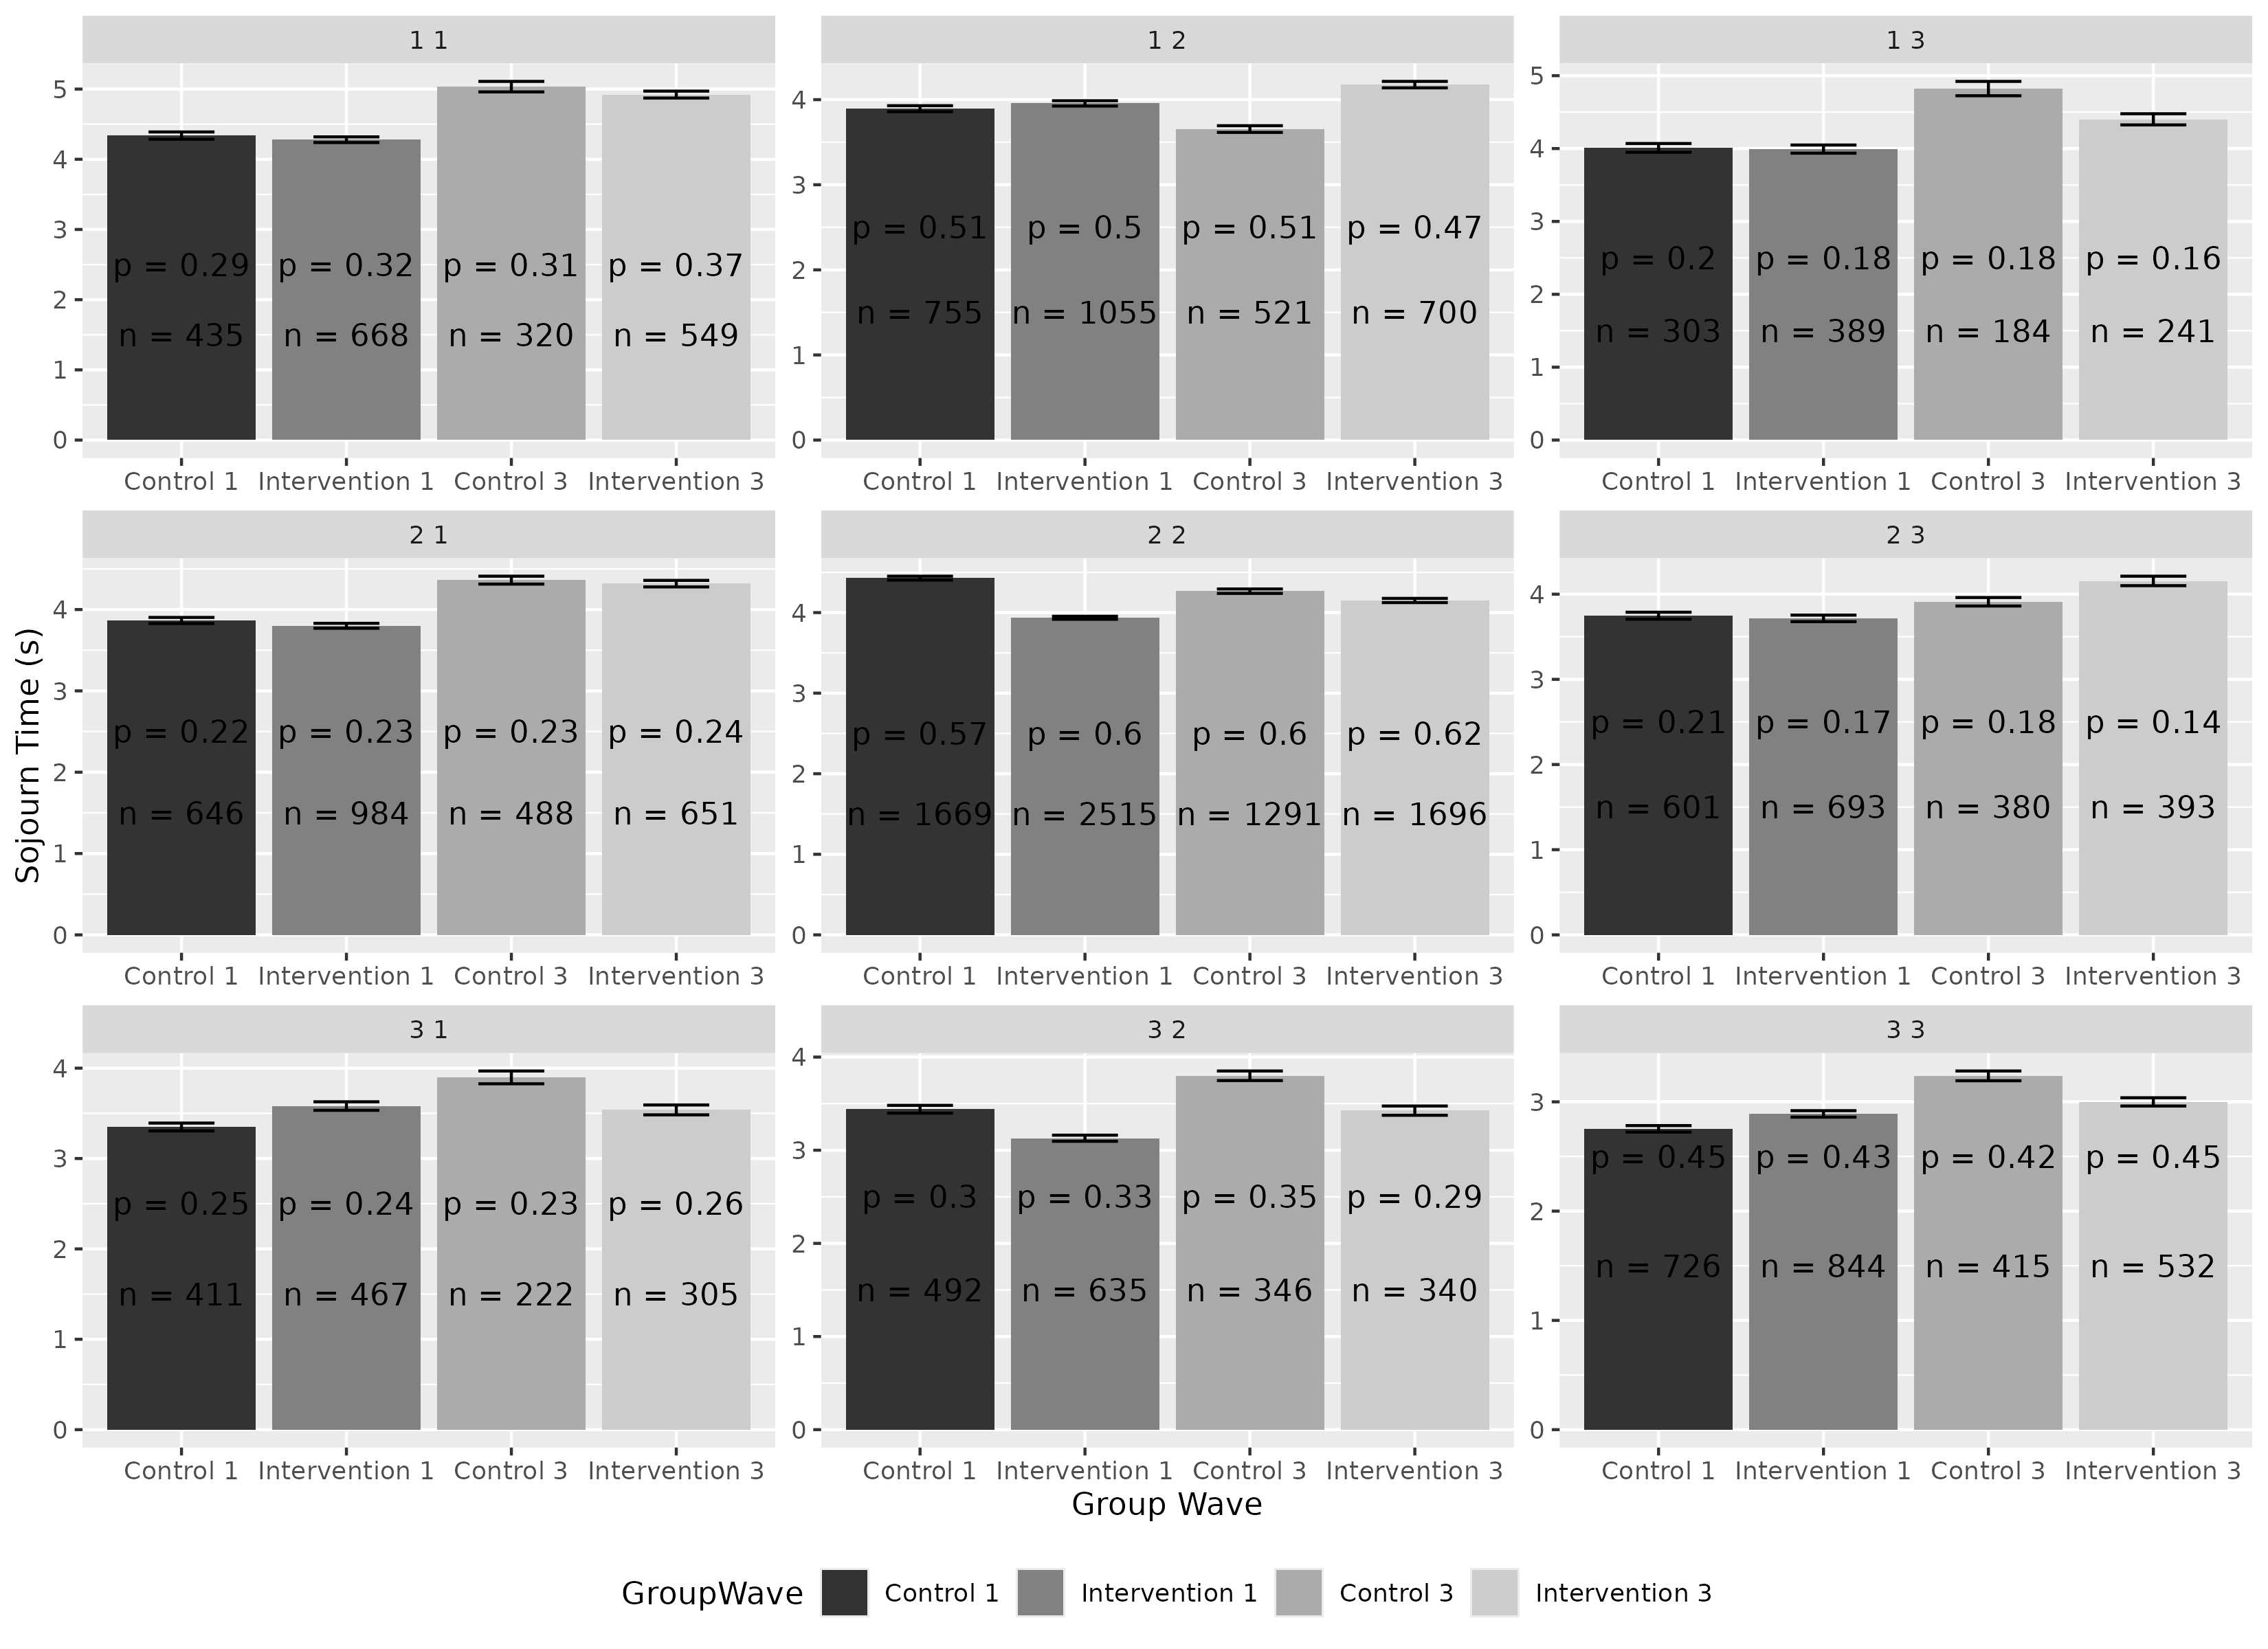
\includegraphics[width=\textwidth,height=2.8125in]{figures/generalSojournTimes.png}
\end{frame}

\begin{frame}{Results cont.}
\phantomsection\label{results-cont.}
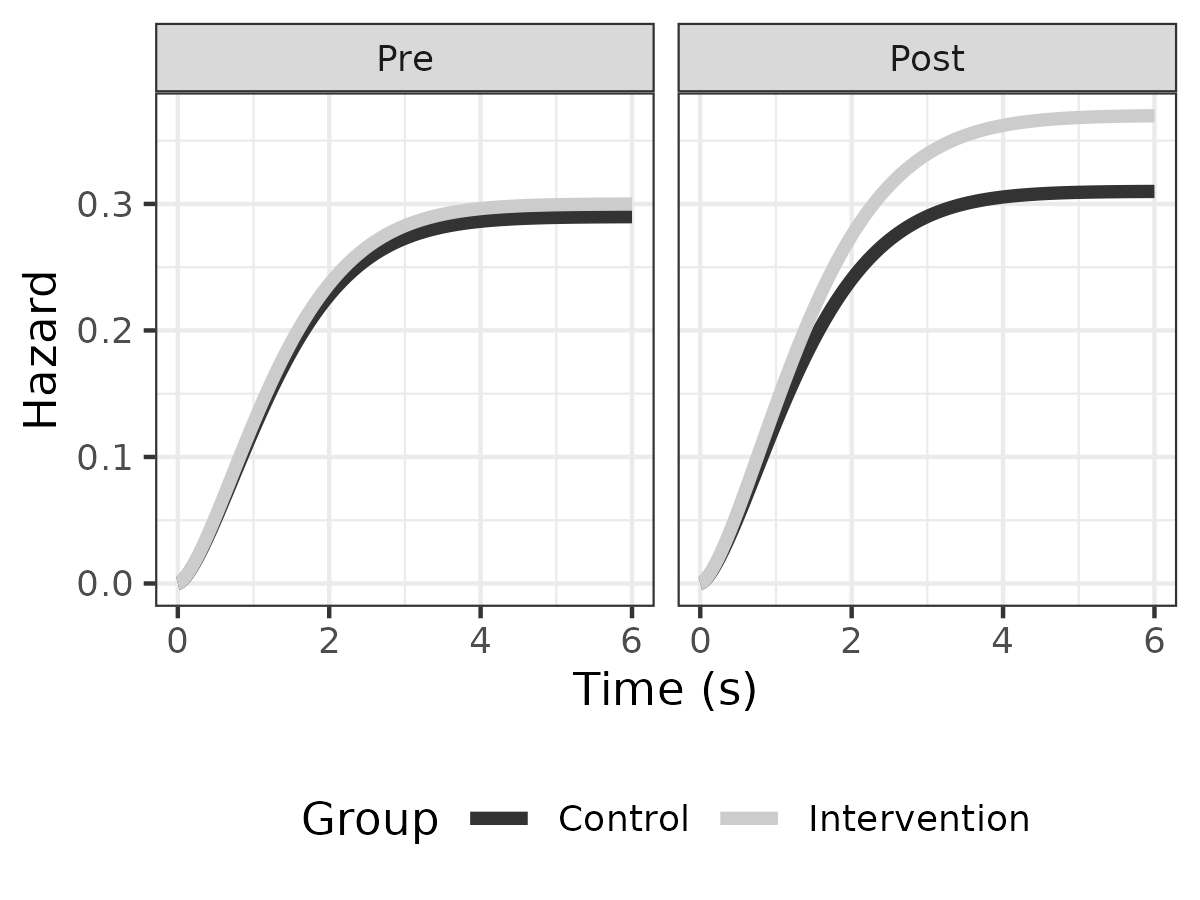
\includegraphics[width=\textwidth,height=3.125in]{figures/allTransOnetoOne.png}
\end{frame}

\begin{frame}{Results cont.}
\phantomsection\label{results-cont.-1}
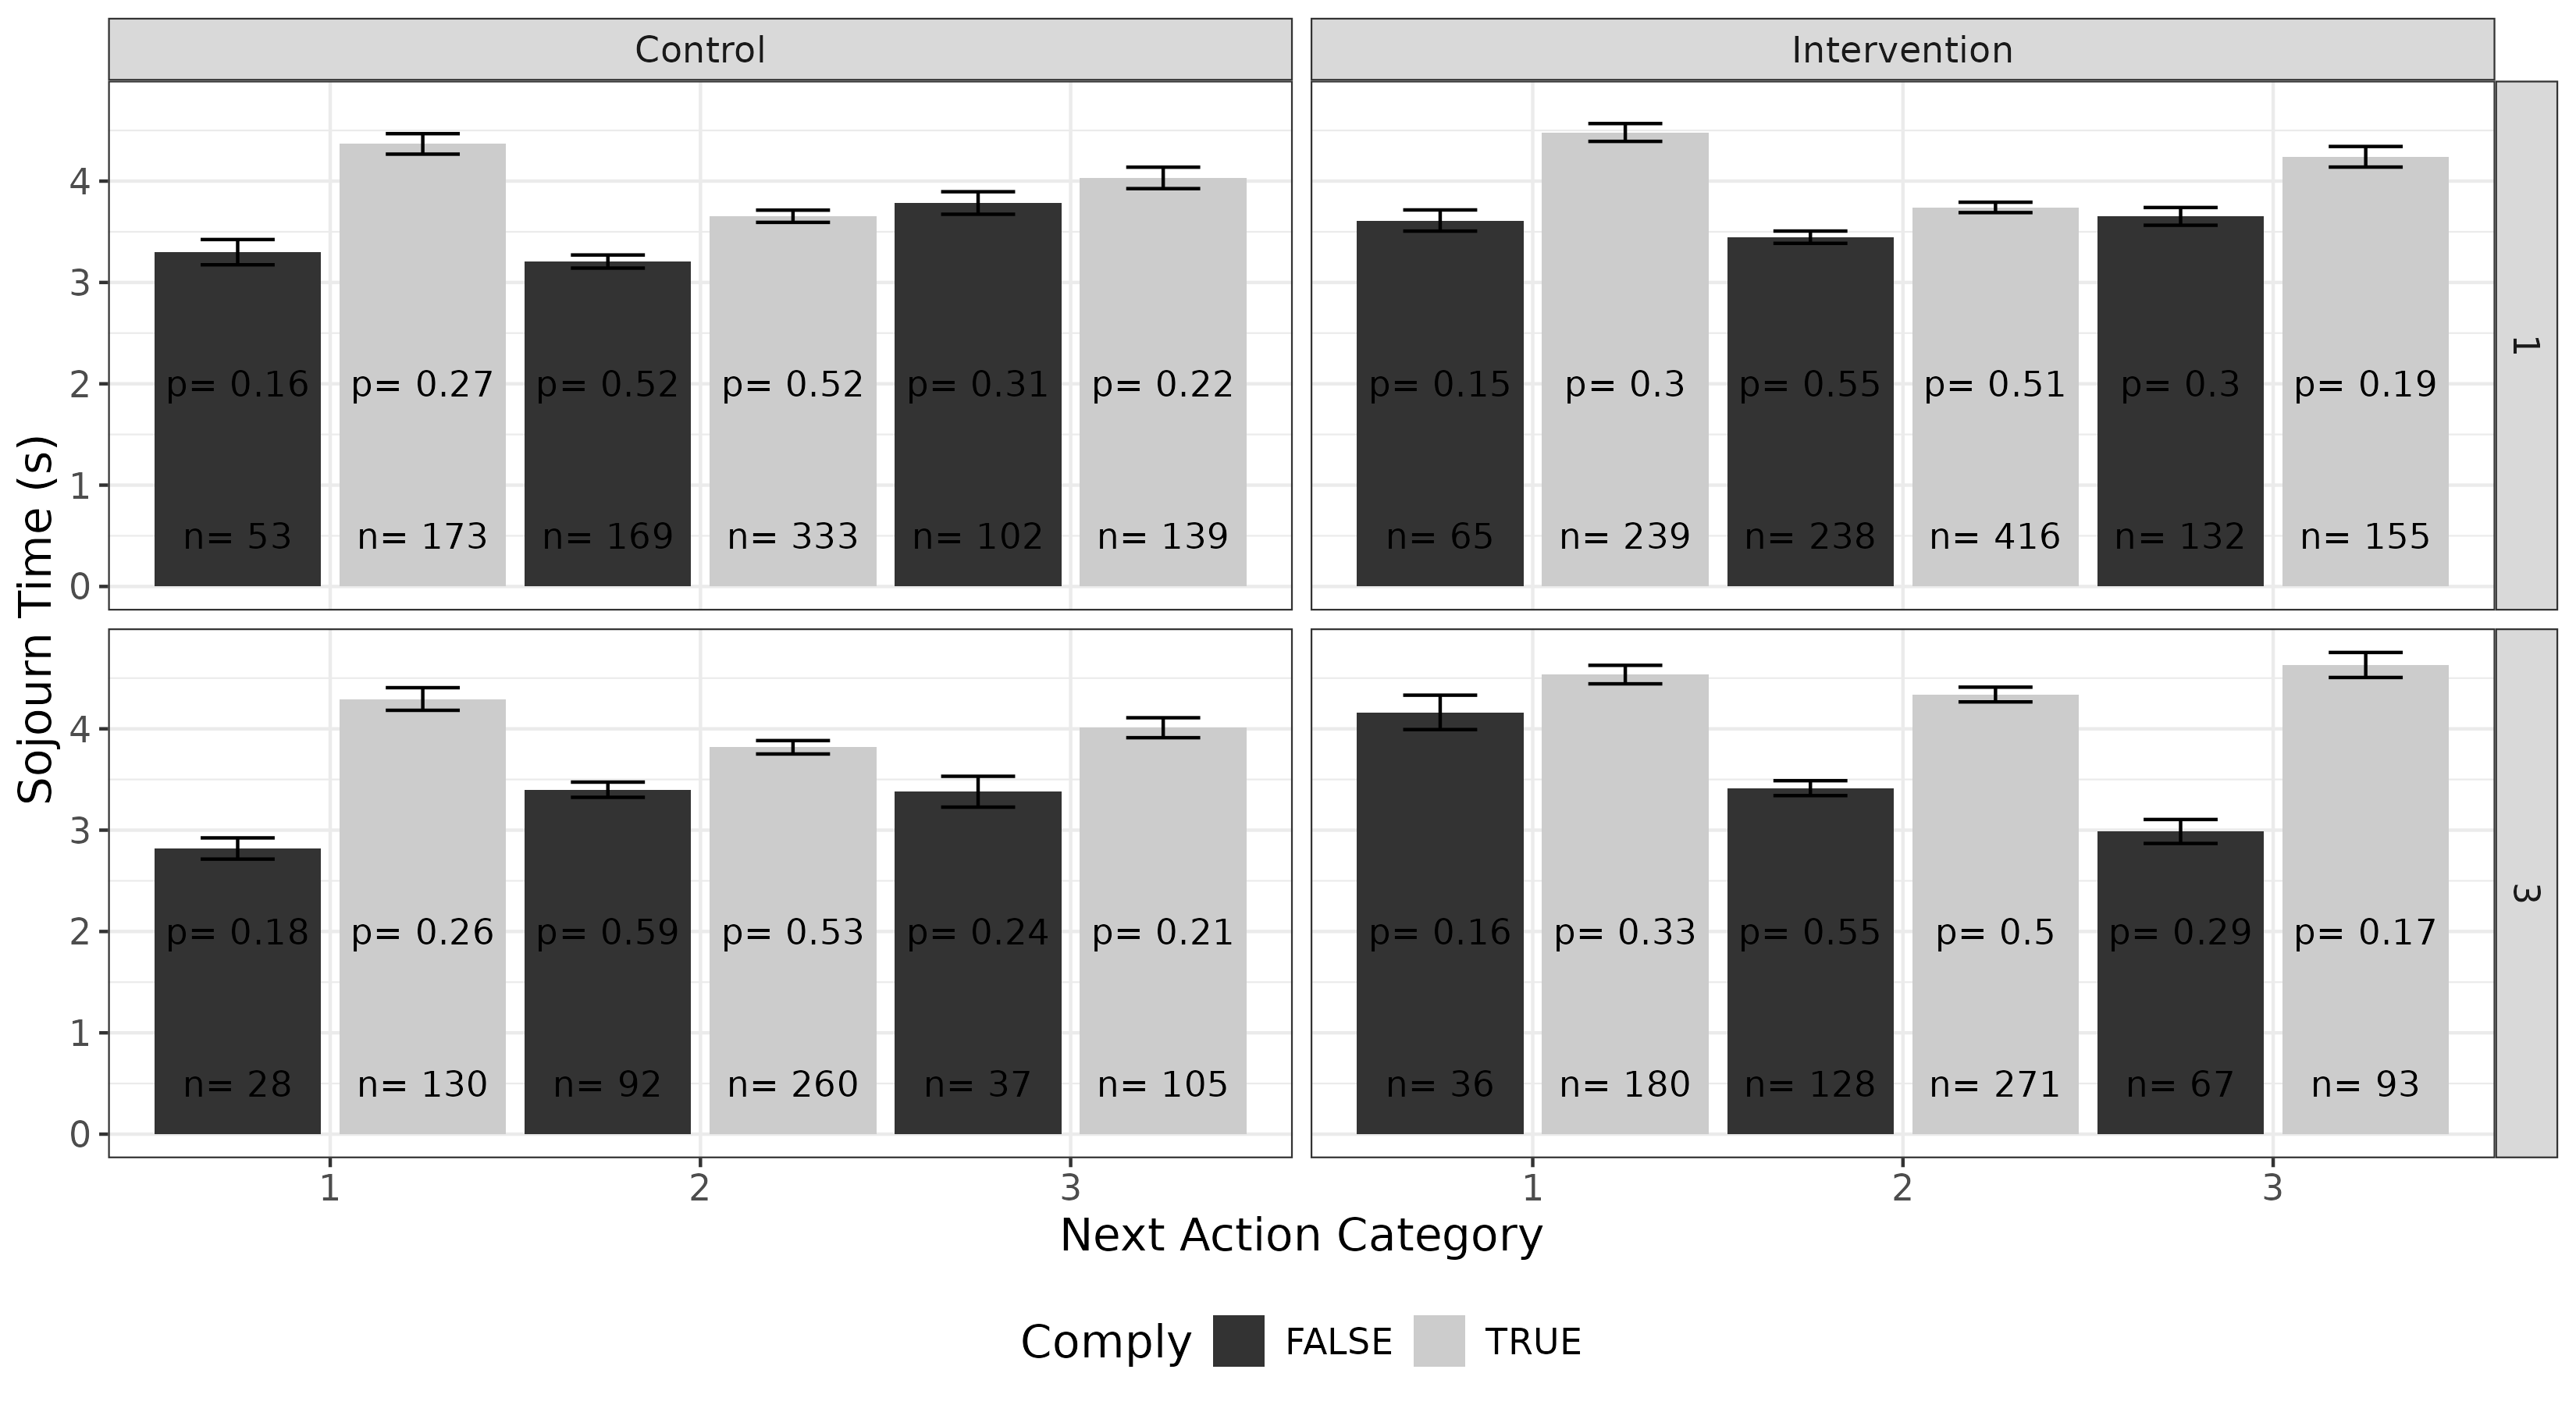
\includegraphics[width=\textwidth,height=3.125in]{figures/complySojournTimes.png}
\end{frame}

\begin{frame}{Results cont.}
\phantomsection\label{results-cont.-2}
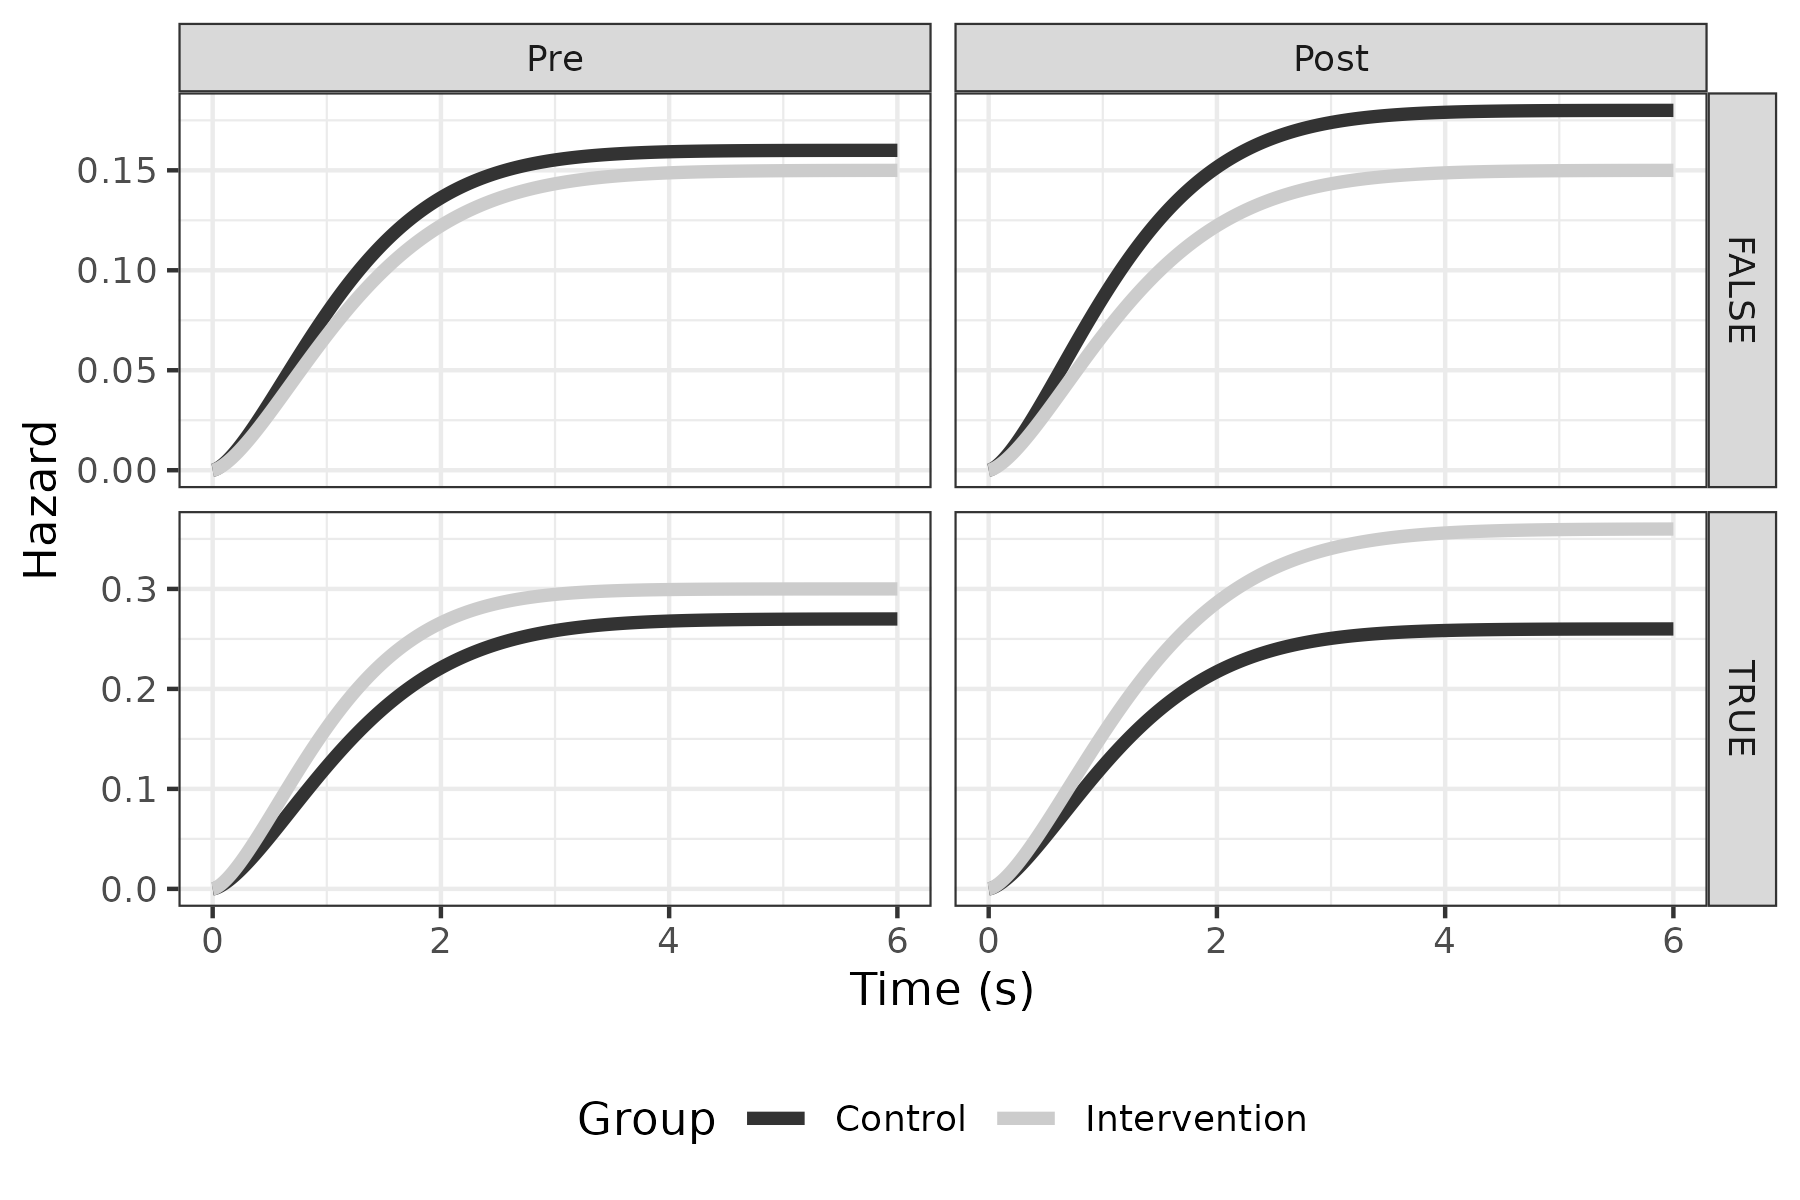
\includegraphics[width=\textwidth,height=3.125in]{figures/complyHazOnetoOne.png}
\end{frame}

\begin{frame}{Empirical Summary}
\phantomsection\label{empirical-summary}
\begin{enumerate}
\item
  PCIT increased the maintenance of the PRIDE state; participants were
  more likely to transition from the PRIDE state into the PRIDE after
  participants were assigned to the intervention cohort; however these
  transitions occurred slower compared to the pre-PCIT DPICS
\item
  PCIT improved PRIDE maintenance a child's compliance; conversely, the
  control cohort displayed reduced timing for PRIDE behaviors after a
  child noncompliance
\end{enumerate}
\end{frame}

\section{Conclusions}\label{conclusions}

\begin{frame}{Conclusions}
\begin{enumerate}
\tightlist
\item
  Semi-Markov models, paramaterized as Multilevel Weibull models, offer
  an attractive alternative to fixed effect Markov models.
\item
  Models that can accommodate population heterogeneity, and non-constant
  hazards reduce error when estimating criterion variables
\item
  The framework proposed here provides a simple alternative to the
  commonly applied discrete-time Markov models that psychologists
  readily apply
\item
  This framework can be used to identify both time variant and
  time-invariant influences of behavioral dynamics as displayed in the
  empirical study performed within this dissertation
\end{enumerate}
\end{frame}

\begin{frame}{Acknowledgments}
\phantomsection\label{acknowledgments}
\begin{columns}[T]
\begin{column}{0.5\textwidth}
\begin{itemize}
\item
  Oklahoma Supercomputing Center for Education \& Research (OSCER)

  \begin{itemize}
  \tightlist
  \item
    \includegraphics[width=1.09375in,height=\textheight]{images/Screenshot from 2024-06-02 21-44-03.png}
  \end{itemize}
\item
  University of Oregon: Elizabeth Skowron Ph.D.

  \begin{itemize}
  \tightlist
  \item
    \includegraphics[width=\textwidth,height=0.78125in]{images/elizabeth-01.jpg}
  \item
    \textbf{\emph{The participants and the data collectors}}
  \end{itemize}
\end{itemize}
\end{column}

\begin{column}{0.5\textwidth}
\begin{itemize}
\item
  University of Oklahoma Department of Psychology

  \begin{itemize}
  \tightlist
  \item
    Cohort: Coop, Em, Justine, Justin
  \item
    Quant: Yaqi Li
  \end{itemize}
\item
  University of Oklahoma Health Sciences Center

  \begin{itemize}
  \tightlist
  \item
    Xiaolan Liao Ph.D.
  \end{itemize}
\item
  \textbf{Committee members}
\item
  \textbf{Kailee, Friends, and Family}
\end{itemize}
\end{column}
\end{columns}
\end{frame}

\begin{frame}{Questions?}
\phantomsection\label{questions}
\begin{block}{THANK YOU!}
\phantomsection\label{thank-you}
\end{block}
\end{frame}

\begin{frame}{References}
\phantomsection\label{references}
\newcommand\Fontvi{\fontsize{4}{4.2}\selectfont}
\fontsize{3.75}{4.2}\selectfont

\phantomsection\label{refs}
\begin{CSLReferences}{1}{0}
\bibitem[\citeproctext]{ref-balanTutorialFrailtyModels2020}
Balan, Theodor A, and Hein Putter. 2020. {``A Tutorial on Frailty
Models.''} \emph{Statistical Methods in Medical Research} 29 (11):
3424--54. \url{https://doi.org/10.1177/0962280220921889}.

\bibitem[\citeproctext]{ref-chamberlainAntisocialBehaviorChildren2003}
Chamberlain, Patricia, and Dana K. Smith. 2003. {``Antisocial Behavior
in Children and Adolescents: {The Oregon Multidimensional Treatment
Foster Care} Model.''} In \emph{Evidence-Based Psychotherapies for
Children and Adolescents}, 282--300. New York, NY, US: The Guilford
Press.

\bibitem[\citeproctext]{ref-coxRegressionModelsLifeTables1972}
Cox, D. R. 1972. {``Regression {Models} and {Life-Tables}.''}
\emph{Journal of the Royal Statistical Society. Series B
(Methodological)} 34 (2): 187--220.
\url{https://www.jstor.org/stable/2985181}.

\bibitem[\citeproctext]{ref-deater-deckardSocioeconomicRiskModerates2012}
Deater-Deckard, Kirby, Nan Chen, Zhe Wang, and Martha Ann Bell. 2012.
{``Socioeconomic Risk Moderates the Link Between Household Chaos and
Maternal Executive Function.''} \emph{Journal of Family Psychology} 26
(3): 391--99. \url{https://doi.org/10.1037/a0028331}.

\bibitem[\citeproctext]{ref-eyberg1988}
Eyberg, Sheila. 1988. {``Parent-Child Interaction Therapy: Integration
of Traditional and Behavioral Concerns.''} \emph{Child \& Family
Behavior Therapy} 10 (1): 3346.
\url{https://doi.org/10.1300/J019v10n01_04}.

\bibitem[\citeproctext]{ref-geeraertsRoleParentalSelfregulation2021}
Geeraerts, Sanne B., Joyce Endendijk, Kirby Deater-Deckard, Jorg
Huijding, Marike H. F. Deutz, Carlijn van den Boomen, and Maja Deković.
2021. {``The Role of Parental Self-Regulation and Household Chaos in
Parent-Toddler Interactions: {A} Time-Series Study.''} \emph{Journal of
Family Psychology} 35 (2): 236--46.
\url{https://doi.org/10.1037/fam0000814}.

\bibitem[\citeproctext]{ref-kalbChildDisobedienceNoncompliance2003}
Kalb, Larry M., and Rolf Loeber. 2003. {``Child Disobedience and
Noncompliance: A Review.''} \emph{Pediatrics} 111 (3): 641--52.
\url{https://doi.org/10.1542/peds.111.3.641}.

\bibitem[\citeproctext]{ref-kaplanNonparametricEstimationIncomplete1958}
Kaplan, E. L., and Paul Meier. 1958. {``Nonparametric {Estimation} from
{Incomplete Observations}.''} \emph{Journal of the American Statistical
Association} 53 (282): 457--81.
\url{https://doi.org/10.1080/01621459.1958.10501452}.

\bibitem[\citeproctext]{ref-keileySurvivalAnalysisFamily2005}
Keiley, Margaret K., and Nina C. Martin. 2005. {``Survival {Analysis} in
{Family Research}.''} \emph{Journal of Family Psychology} 19 (1):
142--56. \url{https://doi.org/10.1037/0893-3200.19.1.142}.

\bibitem[\citeproctext]{ref-lougheedMultilevelSurvivalAnalysis2019}
Lougheed, Jessica P., Lizbeth Benson, Pamela M. Cole, and Nilam Ram.
2019. {``Multilevel {Survival Analysis}: {Studying} the {Timing} of
{Children}'s {Recurring Behaviors}.''} \emph{Developmental Psychology}
55 (1): 53--65. \url{https://doi.org/10.1037/dev0000619}.

\bibitem[\citeproctext]{ref-lunkenheimerBreakingCoerciveCycle2016}
Lunkenheimer, Erika, Anna Lichtwarck-Aschoff, Tom Hollenstein, Christine
J. Kemp, and Isabela Granic. 2016. {``Breaking {Down} the {Coercive
Cycle}: {How Parent} and {Child Risk Factors Influence Real-Time
Variability} in {Parental Responses} to {Child Misbehavior}.''}
\emph{Parenting, Science and Practice} 16 (4): 237--56.
\url{https://doi.org/10.1080/15295192.2016.1184925}.

\bibitem[\citeproctext]{ref-millerFiniteMarkovProcesses1952}
Miller, George A. 1952. {``Finite Markov Processes in Psychology.''}
\emph{Psychometrika} 17 (2): 149--67.
\url{https://doi.org/10.1007/BF02288779}.

\bibitem[\citeproctext]{ref-nelsonDyadicParentChild2018}
Nelson, Melanie McDiarmid, and Brian Olsen. 2018. {``Dyadic
{Parent}--{Child Interaction Coding System} ({DPICS}): {An Adaptable
Measure} of {Parent} and {Child Behavior During Dyadic Interactions}.''}
In \emph{Handbook of {Parent-Child Interaction Therapy}: {Innovations}
and {Applications} for {Research} and {Practice}}, edited by Larissa N.
Niec, 285--302. Cham: Springer International Publishing.
\url{https://doi.org/10.1007/978-3-319-97698-3_18}.

\bibitem[\citeproctext]{ref-owenEffectPraisePositive2012}
Owen, Daniela J., Amy M. S. Slep, and Richard E. Heyman. 2012. {``The
Effect of Praise, Positive Nonverbal Response, Reprimand, and Negative
Nonverbal Response on Child Compliance: A Systematic Review.''}
\emph{Clinical Child and Family Psychology Review} 15 (4): 364--85.
\url{https://doi.org/10.1007/s10567-012-0120-0}.

\bibitem[\citeproctext]{ref-shiffmanEcologicalMomentaryAssessment2008}
Shiffman, Saul, Arthur A. Stone, and Michael R. Hufford. 2008.
{``Ecological Momentary Assessment.''} \emph{Annual Review of Clinical
Psychology} 4: 1--32.
\url{https://doi.org/10.1146/annurev.clinpsy.3.022806.091415}.

\bibitem[\citeproctext]{ref-somersAntecedentsConsequencesChild2024}
Somers, Jennifer A., Kelsey Stiles, Gabrielle A. MacNaughton, Sara J.
Schiff, Yixuan Shen, and Steve S. Lee. 2024. {``Antecedents and
{Consequences} of {Child Externalizing Problems}: {Differences} in
{Dynamic Parent}--{Child Processes}.''} \emph{Research on Child and
Adolescent Psychopathology} 52 (1): 7--19.
\url{https://doi.org/10.1007/s10802-023-01045-0}.

\bibitem[\citeproctext]{ref-standevelopmentteamStanModelingLanguage2023}
Team, Stan Development. 2023. {``Stan {Modeling Language Users Guide}
and {Reference Manual}, 2.34.''}

\end{CSLReferences}
\end{frame}

\end{document}
